\documentclass[11pt, a4paper, titlepage]{report}
\usepackage{amsmath}
\usepackage{natbib}
\usepackage{a4wide}
\usepackage{url}
\usepackage{multirow}
\usepackage{amsfonts}
\usepackage{graphicx}

\newcommand{\release}{4.3.0}
\newcommand{\JAGS}{\textsf{JAGS}}
\newcommand{\rjags}{\textsf{rjags}}
\newcommand{\BUGS}{\textsf{BUGS}}
\newcommand{\OpenBUGS}{\textsf{OpenBUGS}}
\newcommand{\R}{\textsf{R}}
\newcommand{\CODA}{\textsf{coda}}

\begin{document}

\title{JAGS Version \release\ user manual}
\author{Martyn Plummer}
\date{15 May 2017}
\maketitle

\tableofcontents

\chapter{Introduction}

JAGS is Just Another Gibbs Sampler.  It is a program for the analysis
of Bayesian models using Markov Chain Monte Carlo (MCMC) which is not
wholly unlike
\OpenBUGS\ (\url{http://www.openbugs.info}). \JAGS\ was written
with three aims in mind: to have an engine for the \BUGS\ language
that runs on Unix; to be extensible, allowing users to write their own
functions, distributions, and samplers; and to be a platform for
experimentation with ideas in Bayesian modelling.

\JAGS\ is designed to work closely with the \R\ language and
environment for statistical computation and graphics
(\url{http://www.r-project.org}).  You will find it useful to install
the \CODA\ package for \R\ to analyze the output. You can also use the
\rjags\ package to work directly with \JAGS\ from within R (but note
that the \rjags\ package is not described in this manual).

\JAGS\ is licensed under the GNU General Public License
version 2. You may freely modify and redistribute it under certain
conditions (see the file \texttt{COPYING} for details).

\chapter{Running a model in \JAGS}

\JAGS\ is designed for inference on Bayesian models using Markov Chain
Monte Carlo (MCMC) simulation.  Running a model refers to generating
samples from the posterior distribution of the model parameters.  This
takes place in five steps:
\begin{enumerate}
\item Definition of the model
\item Compilation
\item Initialization
\item Adaptation and burn-in
\item Monitoring
\end{enumerate}
The next stages of analysis are done outside of \JAGS: convergence
diagnostics, model criticism, and summarizing the samples must be done
using other packages more suited to this task. There are several
\R\ packages designed for analyzing MCMC output, and \JAGS\ can be
used from within \R\ using the \rjags\ package.

\section{Definition}

There are two parts to the definition of a model in \JAGS: a
description of the model and the definition of the data.

\subsection{Model definition}

The model is defined in a text file using a dialect of the
\BUGS\ language.  The model definition consists of a series of
relations inside a block delimited by curly brackets \verb+{+ and
\verb+}+ and preceded by the keyword \verb+model+. Here is the standard
linear regression example:

\begin{verbatim}
model {
    for (i in 1:N) {
          Y[i]   ~ dnorm(mu[i], tau)
          mu[i] <- alpha + beta * (x[i] - x.bar)
    }
    x.bar   <- mean(x)
    alpha    ~ dnorm(0.0, 1.0E-4)
    beta     ~ dnorm(0.0, 1.0E-4)
    sigma   <- 1.0/sqrt(tau)
    tau      ~ dgamma(1.0E-3, 1.0E-3)
}
\end{verbatim}

\subsubsection{Relations}

Each relation defines a node in the model in terms of other nodes that
appear on the right hand side. These are referred to as the parent
nodes. Taken together, the nodes in the model (together with the
parent/child relationships represented as directed edges) form a
directed acyclic graph. The very top-level nodes in the graph, with no
parents, are constant nodes, which are defined either in the model
definition ({\em e.g.}  \verb+1.0E-3+), or in the data file ({\em
  e.g.}  \verb+x[1]+).

Relations can be of two types. A {\em stochastic relation} (\verb+~+)
defines a stochastic node, representing a random variable in the
model. A {\em deterministic relation} (\verb+<-+) defines a
deterministic node, the value of which is determined exactly by the
values of its parents.

\subsubsection{Parameters and arguments}

Deterministic nodes do not need to be embedded in node arrays. The
node \verb+Y[i]+ could equivalently be defined as
\begin{verbatim}
Y[i] ~ dnorm(alpha + beta * (x[i] - x.bar), tau)
\end{verbatim}

\subsubsection{Arrays and subsetting}

Nodes defined by a relation are embedded in named arrays. Arrays can
be vectors (one-dimensional), or matrices (two-dimensional), or they
may have more than two dimensions.

Array names may contain letters, numbers, decimal points and
underscores, but they must start with a letter.  In the code example
above, the node array \verb+mu+ is a vector of length $N$ containing
$N$ nodes (\verb+mu[1]+, $\ldots$, \verb+mu[N]+). The node array
\verb+alpha+ is a scalar.  \JAGS\ follows the S language convention
that scalars are considered as vectors of length 1. Hence the array
\verb+alpha+ contains a single node \verb+alpha[1]+.

Subsets of node arrays may be obtained with expressions of the form
\verb+alpha[e]+ where \verb+e+ is any expression that evaluates to an
integer vector. Typically expressions of the form \verb+L:U+ are used,
where $L$ and $U$ are integer arguments to the operator $:$. This
creates an integer vector of length $U - L + 1$ with elements $L, L+1,
\ldots U-1, U$.\footnote{If $L > U$ then the operator $:$ returns a
  vector of length zero, which may not be used to take array subsets}
Both the arguments $L$ and $U$ must be fixed because JAGS does not
allow the length of a node to change from one iteration to the next.

Vectors can be constructed using the combine function \texttt{c} from
the \textsf{bugs} module, {\em  e.g.}
\begin{verbatim}
y <- c(x1, x2, x3)
\end{verbatim}
creates a new vector $y$ combining the elements of $x1$, $x2$, and $x3$.    

For a two-dimensional array \verb+B+, the element in row $r$ and
column $c$ is accessed as \verb+B[r,c]+. Complex subsets may be
obtained with expressions of the form \verb+B[rows, cols]+ where
\verb+rows+ is an integer vector of row indices and \verb+cols+ is an
integer vector of column indices.  An index expression in any
dimension may be omitted, and this implies taking the whole range of
possible indices. So if \verb+B+ is an $M \times N$ matrix then
\verb+B[r,]+ is the whole of row $r$, and is equivalent to
\verb+B[r,1:N]+. Likewise \verb+B[,c]+ is the whole of column $c$ and
is equivalent to \verb+B[1:M,c]+. Finally, \verb+B[,]+ is the whole
matrix, equivalent to \verb+B[1:M,1:N]+. In this case, one may also
simply write \verb+B+ without any square brackets. Note that writing
\verb+B[]+ for a 2-dimensional array will result in a compilation
error: the number of indices separated by commas within the square
brackets must match the dimensions of the array.

The combine function can be used with a single array argument
\begin{verbatim}
v <- c(a)
\end{verbatim}
In this case the return value $v$ is a vector with the values of the
input array $a$ in column-major order (i.e. with the left hand index
moving fastest). For example if $a$ is a $2 \times 2$ matrix then
this is equivalent to
\begin{verbatim}
v <- c(a[1,1], a[2,1], a[1,2], a[2,2])
\end{verbatim}

There are some restrictions on index expressions that are allowed on
the left hand side of a relation. Firstly, they must be fixed, meaning
that they must be expressed in terms of data, or constants defined in
the model, or the index of an enclosing for loop (see below).  As
a counter-example, the following code snippet is illegal:
\begin{verbatim}
     i ~ dcat(p)
   x[i] ~ dnorm(0, 1)

\end{verbatim}
unless $i$ is observed and is supplied with the data. This restriction
ensures that the node \verb+x[i]+ can be unambiguously referred to
elsewhere in the model -- e.g. as a function argument or the parameter
for a distribution -- and does not change from one iteration to
another. Secondly, for vector-valued subsets, the same index must not
be repeated. For example, supposed $\mu$ is a 2-vector and $T$ is a
$2 \times 2$ matrix. Then \verb+dmnorm(mu, T)+ defines a bivariate
normal random variable.  However, this code snippet is illegal:
\begin{verbatim}
   indices <- c(1,1)
   x[indices] ~ dmnorm(mu, T)
\end{verbatim}
as it implies writing two different values to the same element \verb+x[1]+.

\subsubsection{For loops}
\label{section:forloops}

Node arrays can be traversed with for loops. 
A general expression for a for loop takes the form
\begin{verbatim}
for (i in exp) {
}
\end{verbatim}
where \texttt{exp} is any expression that evaluates to an integer
vector. The contents of the for loop inside the curly braces will then
be expanded with the index \texttt{i} taking each value in the vector
\texttt{exp}. For example
\begin{verbatim}
for (i in 1:3) {
   Y[i] ~ dnorm(mu, tau)
}
\end{verbatim}
is equivalent to
\begin{verbatim}
Y[1] ~ dnorm(mu, tau)
Y[2] ~ dnorm(mu, tau)
Y[3] ~ dnorm(mu, tau)
\end{verbatim}
As in the above example, for loops generally use the sequence operator
\verb+:+ to generate an increasing sequence of integers. This operator
has high precedence, so is important to use brackets to ensure that
the expression is interpreted correctly. For example, to get a for
loop from $1$ to $m-1$ the correct expression is
\begin{verbatim}
for (i in 1:(m+1)) {
}
\end{verbatim}
Omitting the brackets as in the following expression:
\begin{verbatim}
for (i in 1:m+1) {
}
\end{verbatim}
gives a for loop from $2$ to $m+1$.

The sequence operator \verb+:+ can only produce increasing sequences
(See section \label{base:functions}). If $n < m$ then \verb+m:n+
produces a vector of length zero and when this is used in a for loop
index expression the contents of loop inside the curly brackets are
skipped. Note that this behaviour is different from the sequence
operator in R, where \verb+m:n+ will produce a {\em decreasing}
sequence if $n < m$.

\subsection{Data}
\label{section:data}

The data are defined in a separate file from the model definition, in
the format created by the \texttt{dump()} function in \R (See appendix
\ref{appendix:data}).  Data values may be supplied for stochastic
nodes and constants (including constant values used inside for
loops). It is an error to supply a data value for a deterministic
node. (See, however, section \ref{section:obfun} on observable
functions).

Here are the data for the \verb+LINE+ example:
\begin{verbatim}
`x` <- c(1, 2, 3, 4, 5)
#R-style comments, like this one, can be embedded in the data file
`Y` <- c(1, 3, 3, 3, 5)
`N` <- 5
\end{verbatim}

The unobserved stochastic nodes are referred to as the {\em
  parameters} of the model. The data file therefore defines the
parameters of the model by omission. In the \verb+LINE+ example, the
parameters are \texttt{alpha}, \texttt{beta} and \texttt{tau}.

If a node array contains both observed and unobserved nodes, then the
data should contain missing values (\texttt{NA}) for the unobserved
elements. In the \verb+LINE+ example, if \verb+Y[2]+ and \verb+Y[5]+
were unobserved, then the data would be
\begin{verbatim}
`Y` <- c(1, NA, 3, 3, NA)
\end{verbatim}
Multivariate nodes cannot be partially observed, so if a node takes up
two or more elements of a node array, then the corresponding data
values must be all present or all missing.

\subsection{Node Array dimensions}

\subsubsection*{Array declarations}

\JAGS\ allows the option of declaring the dimensions of node arrays in
the model file. The declarations consist of the keyword \texttt{var}
(for variable) followed by a comma-separated list of array names, with
their dimensions in square brackets. The dimensions may be given in
terms of any expression of the data that returns a single integer
value.

In the linear regression example, the model block could be preceded by
\begin{verbatim}
var x[N], Y[N], mu[N], alpha, beta, tau, sigma, x.bar;
\end{verbatim}

\subsubsection*{Undeclared nodes}

If a node array is not declared then JAGS has three methods of
determining its size.
\begin{enumerate}
\item {\bf Using the data.}  The dimension of an undeclared node array
  may be inferred if it is supplied in the data file.
\item {\bf Using the left hand side of the relations.}  The maximal
  index values on the left hand side of a relation are taken to be the
  dimensions of the node array.  For example, in this case:
\begin{verbatim}
for (i in 1:N) {
   for (j in 1:M) {
      Y[i,j] ~ dnorm(mu[i,j], tau)
   }
}
\end{verbatim}
$Y$ would be inferred to be an $N \times M$ matrix. This method cannot 
be used when there are empty indices ({\em e.g.} \verb+Y[i,]+) on the left
hand side of the relation.
\item {\bf Using the dimensions of the parents} If a whole node array
  appears on the left hand side of a relation, then its dimensions can
  be inferred from the dimensions of the nodes on the right hand side.
  For example, if \verb+A+ is known to be an $N \times N$ matrix
  and
\begin{verbatim}
B <- inverse(A)
\end{verbatim}
Then \verb+B+ is also an $N \times N$ matrix.
\end{enumerate}

\subsubsection*{Querying array dimensions}  

The \JAGS\ compiler has two built-in functions for querying array
sizes.  The \verb+length()+ function returns the number of elements in
a node array, and the \verb+dim()+ function returns a vector
containing the dimensions of an array.  These two functions may be
used to simplify the data preparation. For example, if \verb+Y+
represents a vector of observed values, then using the \verb+length()+
function in a for loop:
\begin{verbatim}
for (i in 1:length(Y)) {
    Y[i] ~ dnorm(mu[i], tau)
}
\end{verbatim}
avoids the need to put a separate data value \verb+N+ in the file
representing the length of \verb+Y+.  

For multi-dimensional arrays, the \verb+dim+ function serves a similar
purpose. The \verb+dim+ function returns a vector, which must be stored
in an array before its elements can be accessed. For this reason, calls
to the \verb+dim+ function must always be in a data block (see section
\ref{section:data:tranformations}).
\begin{verbatim}
data {
   D <- dim(Z)
}
model {
   for (i in 1:D[1]) {
      for (j in 1:D[2]) {
         Z[i,j] <- dnorm(alpha[i] + beta[j], tau)
      }
   }
   ...
}
\end{verbatim}
Clearly, the \verb+length()+ and \verb+dim()+ functions can only
work if the size of the node array can be inferred, using one of the
three methods outlined above.

Note: the \verb+length()+ and \verb+dim()+ functions are different
from all other functions in \JAGS: they do not act on nodes, but only
on node {\em arrays}. As a consequence, an expression such as
\verb+dim(a %*% b)+ is syntactically incorrect.

\section{Compilation}

When a model is compiled, a graph representing the model is created in
computer memory. Compilation can fail for a number of reasons:
\begin{enumerate}
\item The graph contains a directed cycle.  These are forbidden
in \JAGS.
\item A top-level parameter is undefined. Any node that is used on
the right hand side of a relation, but is not defined on the left
hand side of any relation, is assumed to be a constant node. Its value
must be supplied in the data file. 
\item The model uses a function or distribution that has not been
defined in any of the loaded modules.
\end{enumerate}
The number of parallel chains to be run by \JAGS\ is also defined at
compilation time.  Each parallel chain should produce an independent
sequence of samples from the posterior distribution. By default,
\JAGS\ only runs a single chain.

\section{Initialization}

Before a model can be run, it must be initialized. There are three
steps in the initialization of a model:
\begin{enumerate}
\item The initial values of the model parameters are set.
\item A Random Number Generator (RNG) is chosen for each parallel chain,
  and its seed is set.
\item The Samplers are chosen for each parameter in the model. 
\end{enumerate}

\subsection{Parameter values}

The user may supply initial value files -- one for each chain --
containing initial values for the model parameters. The files may not
contain values for logical or constant nodes. The format is the same
as the data file (see (See appendix \ref{appendix:data}).
Section \ref{parameters:in} describes how to read the initial value
files into the model.

As with the data file, you may supply missing values in the initial
values file.  This need typically arises with contrast parameters.
Suppose $X$ is a categorical covariate taking values from 1 to
4. There is one parameter for each level of x ($\beta_1 \ldots
\beta_4$) , but the first parameter $\beta_1$ is set to zero for
identifiability. The remaining parameters $\beta_2 \ldots \beta_4$
represent contrasts with respect to the first level of $X$.
\begin{verbatim}
for (i in 1:N) {
   Y[i] ~ alpha + beta[x[i]]
}
# Prior distribution
alpha ~ dnorm(0, 1.0E-3)
beta[1] <- 0
for(i in 2:4) {
   beta[i] ~ dnorm(0, 1.0E-3)
}
\end{verbatim}
A suitable initial value for \verb+beta+ would be
\begin{verbatim}
`beta` <- c(NA, 1.03, -2.03, 0.52)
\end{verbatim}
This allows parameter values to be supplied for the stochastic
elements of \verb+beta+ but not the constant first element.

If initial values are not supplied by the user, then each parameter
chooses its own initial value based on the values of its parents.  The
initial value is chosen to be a ``typical value'' from the prior
distribution. The exact meaning of ``typical value'' depends on the
distribution of the stochastic node, but is usually the mean, median,
or mode.

If you rely on automatic initial value generation and are running
multiple parallel chains, then the initial values will be the same in
all chains.  You may not want this behaviour, especially if you are
using the Gelman and Rubin convergence diagnostic, which assumes that
the initial values are over-dispersed with respect to the posterior
distribution. In this case, you are advised to set the starting values
manually using the "parameters in" statement.

\subsection{RNGs}
\label{section:rngs}

Each chain in \JAGS\ has its own random number generator (RNG). RNGs
are more correctly referred to as {\em pseudo}-random number
generators. They generate a sequence of numbers that merely looks
random but is, in fact, entirely determined by the initial state.  You
may optionally set the name of the RNG and its initial state in the
initial values file.

The name of the RNG is set as follows. 
\begin{verbatim}
.RNG.name <- "name"
\end{verbatim}
There are four RNGs supplied by the \texttt{base} module in \JAGS\
with the following names:
\begin{verbatim}
"base::Wichmann-Hill"
"base::Marsaglia-Multicarry"
"base::Super-Duper"
"base::Mersenne-Twister"
\end{verbatim}

There are two ways to set the starting state of the RNG. The simplest
is to supply an integer value to \texttt{.RNG.seed}, {\em e.g.}
\begin{verbatim}
".RNG.seed" <- 314159
\end{verbatim}
The second is way to save the state of the RNG from one JAGS session
(see the ``PARAMETERS TO'' statement, section \ref{parameters:to}) and
use this as the initial state of a new chain. The state of any RNG in
JAGS can be saved and loaded as an integer vector with the name
\texttt{.RNG.state}. For example,
\begin{verbatim}
".RNG.state" <- as.integer(c(20899,10892,29018))
\end{verbatim}
is a valid state for the Marsaglia-Multicarry generator.  You cannot
supply an arbitrary integer to \texttt{.RNG.state}. Both the length of
the vector and the permitted values of its elements are determined by
the class of the RNG. The only safe way to use \texttt{.RNG.state} is
to re-use a previously saved state.

If no RNG names are supplied, then RNGs will be chosen automatically
so that each chain has its own independent random number stream.  The
exact behaviour depends on which modules are loaded. The \texttt{base}
module uses the four generators listed above for the first four
chains, then recycles them with different seeds for the next four
chains, and so on.  

By default, \JAGS\ bases the initial state on the time stamp. This
means that, when a model is re-run, it generates an independent set of
samples. If you want your model run to be reproducible, you must
explicitly set the \verb+.RNG.seed+ for each chain.

\subsection{Samplers}

A Sampler is an object that acts on a set of parameters and updates
them from one iteration to the next. During initialization of the
model, Samplers are chosen automatically for all parameters. 

The Model holds an internal list of {\em Sampler Factory} objects,
which inspect the graph, recognize sets of parameters that can be
updated with specific methods, and generate Sampler objects for
them. The list of Sampler Factories is traversed in order, starting with
sampling methods that are efficient, but limited to certain specific
model structures and ending with the most generic, possibly
inefficient, methods. If no suitable Sampler can be generated for one
of the model parameters, an error message is generated.

The user has no direct control over the process of choosing
Samplers. However, you may indirectly control the process by loading a
module that defines a new Sampler Factory. The module will insert the
new Sampler Factory at the beginning of the list, where it will be
queried before all of the other Sampler Factories. You can also 
optionally turn on and off sampler factories using the ``SET FACTORY''
command. See \ref{set:factory}.

A report on the samplers chosen by the model, and the stochastic nodes
they act on, can be generated using the ``SAMPLERS TO'' command. See 
section \ref{samplers:to}.
 
\section{Adaptation and burn-in}

In theory, output from an MCMC sampler converges to the target
distribution ({\em i.e.} the posterior distribution of the model
parameters) in the limit as the number of iterations tends to
infinity. In practice, all MCMC runs are finite.  By convention, the
MCMC output is divided into two parts: an initial ``burn-in'' period,
which is discarded, and the remainder of the run, in which the output
is considered to have converged (sufficiently close) to the target
distribution. Samples from the second part are used to create
approximate summary statistics for the target distribution.

By default, \JAGS\ keeps only the current value of each node in the
model, unless a monitor has been defined for that node. The burn-in
period of a \JAGS\ run is therefore the interval between model
initialization and the creation of the first monitor.

When a model is initialized, it may be in {\em adaptive mode}, meaning
that the Samplers used by the model may modify their behaviour for
increased efficiency. Since this adaptation may depend on the entire
sample history, the sequence generated by an adapting sampler is no
longer a Markov chain, and is not guaranteed to converge to the target
distribution. Therefore, adaptive mode must be turned off at some
point during burn-in, and a sufficient number of iterations must take
place {\em after} the adaptive phase to ensure successful burnin.

By default, adaptive mode is turned off half way through first update
of a \JAGS\ model. All samplers have a built in test to determine
whether they have converged to their optimal sampling behaviour.  If
any sampler fails this validation test, a warning will be printed. To
ensure optimal sampling behaviour, the model should be run again from
scratch using a longer adaptation period.

The \texttt{adapt} command (see section \ref{section:adapt}) can be
used for more control over the adaptive phase.  The \texttt{adapt}
command updates the model but keeps it in adaptive mode. At the end of
each update, the convergence test is called. The message ``Adaptation
successful'' will be printed if the convergence test is successful,
otherwise the message will read ``Adaptation incomplete''.  Successive
calls to \texttt{adapt} are possible while keeping the model in
adaptive mode. The next \texttt{update} command will immediately turn
off adaptive mode.

\section{Monitoring}
\label{section:monitoring}

A {\em monitor} in \JAGS\ is an object that records sampled
values. The simplest monitor is a {\em trace monitor}, which stores
the sampled value of a node at each iteration.

\JAGS\ cannot monitor a node unless it has been defined in the model
file.  For vector- or array-valued nodes, this means that every
element must be defined. Here is an example of a simple for loop that
only defines elements $2$ to $N$ of \verb+theta+

\begin{verbatim}
for (i in 2:N) {
   theta[i] ~ dnorm(0,1);
}
\end{verbatim}

Unless \verb+theta[1]+ is defined somewhere else in the model file,
the multivariate node \verb+theta+ is undefined and therefore it
will not be possible to monitor \verb+theta+ as a whole.  In such
cases you can request each element separately , e.g. \verb+theta[2]+,
\verb+theta[3]+, {\em etc.}, or request a subset that is fully defined,
e.g. \verb+theta[2:6]+.

Monitors can be classified according to whether they pool values over
iterations and whether they pool values over parallel chains (The
standard trace monitor does neither). When monitor values are written
out to file using the CODA command, the output files created depend
on the pooling of the monitor, as shown in table \ref{table:coda}. By
default, all of these files have the prefix CODA, but this may be changed
to any other name using the ``stem'' option to the CODA command
(See \ref{coda}).

\begin{table}[h]
\begin{tabular}{ccl}
\hline
Pool       & Pool   & Output files \\
iterations & chains &              \\
\hline
no         & no     & CODAindex.txt, CODAchain1.txt, ... 
                      CODAchainN.txt \\
no         & yes    & CODAindex0.txt, CODAchain0.txt \\
yes        & no     & CODAtable1.txt, ... CODAtableN.txt \\
yes        & yes    & CODAtable0.txt \\
\hline
\end{tabular}
\caption{Output files created by the CODA command depending on whether
a monitor pools its values over chains or over iterations \label{table:coda}}
\end{table}

The standard CODA format for monitors that do not pool values over
iterations is to create an index file and one or more output files.
The index file is has three columns with, one each line,
\begin{enumerate}
\item A string giving the name of the (scalar) value being recorded
\item The first line in the output file(s)
\item The last line in the output file(s)
\end{enumerate}
The output file(s) contain two columns:
\begin{enumerate}
\item The iteration number
\item The value at that iteration
\end{enumerate}

Some monitors pool values over iterations. For example a mean monitor
may record only the sample mean of a node, without keeping the
individual values from each iteration. Such monitors are written out
to a table file with two columns:
\begin{enumerate}
\item A string giving the name of the (scalar) value being recorded
\item The value (pooled over all iterations)
\end{enumerate}

%Chapter Running JAGS from R

\chapter{Running \JAGS}

\JAGS\ has a command line interface. To invoke jags interactively,
simply type \texttt{jags} at the shell prompt on Unix, a Terminal window on MacOS, or the Windows
command prompt on Windows. To invoke JAGS with a script file, type
\begin{verbatim}
jags <script file>
\end{verbatim}
A typical script file has the following commands: 
\begin{verbatim}
model in "line.bug"      # Read model file
data in "line-data.R"    # Read data in from file
compile, nchains(2)      # Compile a model with two parallel chains
parameters in "line-inits1.R", chain(1) # Read initial values from file for chain 1
parameters in "line-inits2.R", chain(2) # Read initial values from file for chain 2
initialize               # Initialize the model
update 1000              # Adaptation (if necessary) and burnin for 1000 iterations
monitor alpha            # Set trace monitor for node alpha ...
monitor beta             # ... and beta
monitor sigma            # ... and sigma
update 10000             # Update model for 10000 iterations
coda *                   # All monitored values are written out to file
\end{verbatim}
More examples can be found in the file \verb+classic-bugs.tar.gz+
which is available from Sourceforge
(\url{http://sourceforge.net/projects/mcmc-jags/files}.

Output from \JAGS\ is printed to the standard output, even when a
script file is being used.  

\section{Scripting commands}
\label{section:scripting}

\JAGS\ has a simple set of scripting commands with a syntax loosely
based on \textsf{Stata}. Commands are shown below preceded by a dot
(.). This is the \JAGS\ prompt. Do not type the dot in when you are
entering the commands.

C-style block comments taking the form /* ... */ can be
embedded anywhere in the script file.  Additionally, you may use
\R-style single-line comments starting with \#.

If a scripting command takes a file name, then the name may be
optionally enclosed in quotes. Quotes are required when the file name
contains space, or any character which is not alphanumeric, or one of
the following: \verb+_+, \verb+-+, \verb+.+, \verb+/+, \verb+\+.

In the descriptions below, angular brackets \verb+<>+, and the text
inside them, represents a parameter that should be replaced with the
correct value by you.  Anything inside square brackets \verb+[]+ is
optional. Do not type the square brackets if you wish to use an
option.

\subsection{MODEL IN}

\begin{verbatim}
. model in <file>
\end{verbatim}
Checks the syntactic correctness of the model description in
\texttt{file} and reads it into memory. The next compilation
statement will compile this model. 

See also: MODEL CLEAR (\ref{model:clear})

\subsection{DATA IN}
\label{data:in}

\begin{verbatim}
. data in <file>
\end{verbatim}
JAGS keeps an internal data table containing the values of observed
nodes inside each node array.  The DATA IN statement reads data from a
file into this data table.

Several data statements may be used to read in data from more than one
file. If two data files contain data for the same node array, the second
set of values will overwrite the first, and a warning will be printed.

See also: DATA TO (\ref{data:to}).

\subsection{COMPILE}

\begin{verbatim}
. compile [, nchains(<n>)]
\end{verbatim}
Compiles the model using the information provided in the preceding
model and data statements. By default, a single Markov chain is
created for the model, but if the \texttt{nchains} option is given,
then \texttt{n} chains are created 

Following the compilation of the model, further DATA IN statements are
legal, but have no effect.  A new model statement, on the other hand,
will replace the current model.

\subsection{PARAMETERS IN}
\label{parameters:in}

\begin{verbatim}
. parameters in <file> [, chain(<n>)]
\end{verbatim}
Reads the values in \texttt{file} and writes them to the corresponding
parameters in chain \texttt{n}. The file has the same format as the
one in the DATA IN statement.  The \texttt{chain} option may be
omitted, in which case the parameter values in all chains are set to
the same value.

The PARAMETERS IN statement must be used after the COMPILE statement
and before the INITIALIZE statement.  You may only supply the values of
unobserved stochastic nodes in the parameters file, not logical or
constant nodes.

See also: PARAMETERS TO (\ref{parameters:to})

\subsection{INITIALIZE}

\begin{verbatim}
. initialize
\end{verbatim}
Initializes the model using the previously supplied data and parameter
values supplied for each chain.

\subsection{UPDATE}

\begin{verbatim}
. update <n> [,by(<m>)]
\end{verbatim}
Updates the model by \texttt{n} iterations. 

If JAGS is being run interactively, a progress bar is printed on the
standard output consisting of 50 asterisks. If the \texttt{by} option
is supplied, a new asterisk is printed every \texttt{m} iterations. If
this entails more than 50 asterisks, the progress bar will be wrapped
over several lines.  If \texttt{m} is zero, the printing of the
progress bar is suppressed.

If JAGS is being run in batch mode, then the progress bar is
suppressed by default, but you may activate it by supplying the
\texttt{by} option with a non-zero value of \texttt{m}.

If the model has an adaptive sampling phase, the first UPDATE
statement turns off adaptive mode for all samplers in the model after
\texttt{n/2} iterations. A warning is printed if adaptation is
incomplete. Incomplete adaptation means that the mixing of the Markov
chain is not optimal. It is still possible to continue with a model
that has not completely adapted, but it may be preferable to run the
model again with a longer adaptation phase, starting from the MODEL IN
statement. Alternatively, you may use an ADAPT statement (see below)
immediately after initialization.

\subsection{ADAPT}
\label{section:adapt}

\begin{verbatim}
. adapt <n> [,by(<m>)]
\end{verbatim}
Updates the model by \texttt{n} iterations keeping the model in
adaptive mode and prints a message to indicate whether adaptation is
successful.  Successive calls to ADAPT may be made until the
adaptation is successful. The next call to UPDATE then turns off
adaptive mode immediately.

Use this instead of the first UPDATE statement if you want explicit
control over the length of the adaptive sampling phase.

Like the UPDATE statement, the ADAPT statement prints a progress
bar, but with plus signs instead of asterisks.

\subsection{MONITOR}
\label{section:monitor}

In \JAGS, a monitor is an object that calculates summary statistics
from a model.  The most commonly used monitor simply records the value
of a single node at each iteration.  This is called a ``trace''
monitor. 
\begin{verbatim}
. monitor <varname> [, thin(n)] [type(<montype>)]
\end{verbatim}
The \texttt{thin} option sets the thinning interval of the monitor so
that it will only record every nth value. The \texttt{thin} option 
selects the type of monitor to create. The default type is \texttt{trace}.

More complex monitors can be defined that do additional calculations.
For example, the \verb+dic+ module defines a ``deviance'' monitor that
records the deviance of the model at each iteration, and a ``pD''
monitor that calculates an estimate of the effective number of
parameters on the model \citep{spiegelhalter:etal:2002}.  

\begin{verbatim}
. monitor clear <varname> [type(<montype>)]
\end{verbatim}
Clears the monitor of the given type associated with variable
\texttt{<varname>}. 

\subsection{CODA}
\label{coda}

\begin{verbatim}
. coda <varname> [, stem(<filename>)]
\end{verbatim}
If the named node has a trace monitor, this dumps the monitored values
of to files \texttt{CODAindex.txt}, \texttt{CODAindex1.out},
\texttt{CODAindex2.txt}, \ldots in a form that can be read by the
\CODA\ package of \R.  The stem option may be used to modify the
prefix from ``CODA'' to another string.  The wild-card character ``*''
may be used to dump all monitored nodes

\subsection{EXIT}

\begin{verbatim}
. exit
\end{verbatim}
Exits \JAGS. \JAGS\ will also exit when it reads an end-of-file character.

\subsection{DATA TO}
\label{data:to}
\begin{verbatim}
. data to <filename>
\end{verbatim}
Writes the data ({\em i.e.} the values of the observed nodes) to a
file in the R \texttt{dump} format. The same file can be used in a
DATA IN statement for a subsequent model.

See also: DATA IN (\ref{data:in})

\subsection{PARAMETERS TO}
\label{parameters:to}
\begin{verbatim}
. parameters to <file> [, chain(<n>)]
\end{verbatim}
Writes the current parameter values ({\em i.e.} the values of the
unobserved stochastic nodes) in chain \texttt{<n>} to a file in R dump
format. The name and current state of the RNG for chain \texttt{<n>}
is also dumped to the file.  The same file can be used as input in a
PARAMETERS IN statement in a subsequent run.

See also: PARAMETERS IN (\ref{parameters:in})

\subsection{SAMPLERS TO}
\label{samplers:to}
\begin{verbatim}
. samplers to <file>
\end{verbatim}
Writes out a summary of the samplers to the given file.  The output appears
in three tab-separated columns, with one row for each sampled node
\begin{itemize}
\item The index number of the sampler (starting with 1). The index number 
gives the order in which Samplers are updated at each iteration.
\item The name of the sampler, matching the index number
\item The name of the sampled node. 
\end{itemize}
If a Sampler updates multiple nodes then it is represented by multiple rows
with the same index number.

Note that the list includes only those nodes that are updated by a
Sampler.  Stochastic nodes that are updated by forward sampling from
the prior are not listed.

\subsection{LOAD}
\label{load}
\begin{verbatim}
. load <module>
\end{verbatim}
Loads a module into \JAGS\ (see chapter \ref{chapter:modules}). Loading
a module does not affect any previously initialized models, but will
affect the future behaviour of the compiler and model initialization.

\subsection{UNLOAD}
\label{unload}
\begin{verbatim}
. unload <module>
\end{verbatim}
Unloads a module. Currently initialized models are unaffected, but
the functions, distribution, and factory objects in the model will not
be accessible to future models.

\subsection{LIST MODULES}
\label{list:modules}
\begin{verbatim}
. list modules
\end{verbatim}
Prints a list of the currently loaded modules.

\subsection{LIST FACTORIES}
\label{list:factories}
\begin{verbatim}
. list factories, type(<factype>)
\end{verbatim}
List the currently loaded factory objects and whether or not they are
active.  The \verb+type+ option must be given, and the three possible values
of \verb+<factype>+ are \verb+sampler+, \verb+monitor+, and \verb+rng+.

\subsection{SET FACTORY}
\label{set:factory}
\begin{verbatim}
. set factory "<facname>" <status>, type(<factype>)
\end{verbatim}
Sets the status of a factor object. The possible values of \verb+<status>+
are \verb+on+ and \verb+off+. Possible factory names are given from the
LIST MODULES command.

\subsection{MODEL CLEAR}
\label{model:clear}
\begin{verbatim}
. model clear
\end{verbatim}
Clears the current model.  The data table (see section \ref{data:in})
remains intact

\subsection{Print Working Directory (PWD)}
\begin{verbatim}
. pwd
\end{verbatim}
Prints the name of the current working directory. This is where \JAGS\
will look for files when the file name is given without a full path, 
{\em e.g.} \verb+"mymodel.bug"+.

\subsection{Change Directory (CD)}
\begin{verbatim}
. cd <dirname>
\end{verbatim}
Changes the working directory to \texttt{<dirname>}

\subsection{Directory list (DIR)}
\begin{verbatim}
. dir
\end{verbatim}
Lists the files in the current working directory.

\subsection{RUN}
\begin{verbatim}
. run <cmdfile>
\end{verbatim}
Opens the file \texttt{<cmdfile>} and reads further scripting commands
until the end of the file.  Note that if the file contains an EXIT
statement, then the \JAGS\ session will terminate. 


\section{Errors}

There are two kinds of errors in \JAGS: runtime errors, which are due to
mistakes in the model specification, and logic errors which are internal
errors in the JAGS program. 

Logic errors are generally created in the lower-level parts of the \JAGS\
library, where it is not possible to give an informative error message.
The upper layers of the \JAGS\ program are supposed to catch such errors
before they occur, and return a useful error message that will help you
diagnose the problem.  Inevitably, some errors slip through. Hence,
if you get a logic error, there is probably an error in your input to
\JAGS, although it may not be obvious what it is. Please send a bug
report (see ``Feedback'' below) whenever you get a logic error.

Error messages may also be generated when parsing files (model files,
data files, command files).  The error messages generated in this case
are created automatically by the program \texttt{bison}. They
generally take the form ``syntax error, unexpected FOO, expecting BAR''
and are not always abundantly clear.

If a model compiles and initializes correctly, but an error occurs
during updating, then the current state of the model will be dumped
to a file named \verb+jags.dumpN.R+ where $N$ is the chain number.
You should then load the dumped data into R to inspect the state of
each chain when the error occurred.

\chapter{Functions}
\label{section:functions}

Functions allow deterministic nodes to be defined using the \verb+<-+
(``gets'') operator.  Most of the functions in \JAGS\ are scalar
functions taking scalar arguments. However, \JAGS\ also allows
arbitrary vector- and array-valued functions, such as the matrix
multiplication operator \verb+%*%+ and the transpose function
\verb+t()+ defined in the \verb+bugs+ module, and the matrix
exponential function \verb+mexp()+ defined in the \verb+msm+
module. \JAGS\ also uses an enriched dialect of the BUGS language with
a number of operators that are used in the S language.

Scalar functions taking scalar arguments are automatically vectorized.
They can also be called when the arguments are arrays with conforming
dimensions, or scalars. So, for example, the scalar $c$ can be added to
the matrix $A$ using
\begin{verbatim}
B <- A + c
\end{verbatim}
instead of the more verbose form
\begin{verbatim}
D <- dim(A)
for (i in 1:D[1])
   for (j in 1:D[2]) {
      B[i,j] <- A[i,j] + c
   }
}
\end{verbatim}
Inverse link functions are an exception to this rule ({\em i.e.} exp,
icloglog, ilogit, phi) and cannot be vectorized. 

A function may optionally have an alias, which can be used in the
model definition in place of the canonical name. Aliases are used to
to avoid confusion with other software in which functions may have
different names.

\chapter{Distributions}
\label{chapter:distributions}

Distributions are used to define stochastic nodes using the \verb+~+
operator.

Some distributions have restrictions on the valid parameter values,
and these are indicated in the tables. If a distribution is
given invalid parameter values when evaluating the log-likelihood, it
returns $-\infty$. When a model is initialized, all stochastic nodes
are checked to ensure that the initial parameter values are valid for
their distribution.

A distribution may optionally have an alias, which can be used in the
model definition in place of the canonical name. Aliases are used to
avoid confusion with other statistical software in which distributions
may have slightly different names. Note however that the alias does
not change the parameterization. For example, the Weibull distribution
is parameterized differently in BUGS and R, and using the alias
\texttt{dweibull} does not change this.

\section{Functions associated with distributions}

All distributions in JAGS have a log density function associated with
them.  For example, if variable \texttt{x} has a normal distribution
with mean \texttt{mu} and precision \texttt{tau}:
\begin{verbatim}
x ~ dnorm(mu, tau)
\end{verbatim}
then the log density of \texttt{x} is given by
\begin{verbatim}
ldx <- logdensity.norm(x, mu, tau)
\end{verbatim}
In general, if ``\texttt{dfoo}'' is the name of a distribution then
the associated log density function is
``\texttt{logdensity.foo}''. The first argument of the log-density
function is the sample value at which the log-density is evaluated and
the remaining arguments are the parameters of the distribution.

For some scalar-valued distributions, additional functions are
available that give the probability density, probability function and
the quantile function. These distributions and associated functions
are given in table~\ref{table:dpq}. These distributions are all in the
\texttt{bugs} module. See section \ref{section:bugs:distributions} for
details on the parameterization of these distributions.

The density, probability, and quantile functions associated with the
normal distribution are illustrated below:
\begin{verbatim}
density.x  <- dnorm(x, mu, tau)     # Density of normal distribution at x
prob.x     <- pnorm(x, mu, tau)     # P(X <= x)
quantile90.x <- qnorm(0.9, mu, tau) # 90th percentile
\end{verbatim}

\begin{table}
\begin{center}
\begin{tabular}{llll}
\hline
Distribution & Distribution & Quantile \\
\hline
Bernoulli          & dbern     & pbern     & qbern \\
Beta               & dbeta     & pbeta     & qbeta \\
Binomial           & dbin      & pbin      & qbin \\
Chi-squared        & dchisqr   & pchisqr   & qchisqr \\
Double exponential & ddexp     & pdexp     & qdexp \\
Exponential        & dexp      & pexp      & qexp \\
F                  & df        & pf        & qf \\
Gamma              & dgamma    & pgamma    & qgamma \\
Generalized gamma  & dgen.gamma & pgen.gamma & qgen.gamma \\
Noncentral hypergeometric     & dhyper    & phyper    & qhyper \\
Logistic           & dlogis    & plogis    & qlogis \\
Log-normal         & dlnorm    & plnorm    & qlnorm \\
Negative binomial  & dnegbin   & pnegbin   & qnegbin \\
Noncentral Chi-squared & dnchisqr   & pnchisqr   & qnchisqr \\
Normal             & dnorm     & pnorm     & qnorm \\
Pareto             & dpar      & ppar      & qpar \\
Poisson            & dpois     & ppois     & qpois \\
Student t          & dt        & pt        & qt \\
Weibull            & dweib     & pweib     & qweib \\
\hline
\end{tabular}
\caption{Functions to calculate the probability density, probability
  function, and quantiles of some of the distributions provided by the
  \texttt{bugs} module. \label{table:dpq}}
\end{center}
\end{table}

\subsection{Observable Functions}
\label{section:obfun}

Logical nodes in the \BUGS\ language are a convenient way of
describing the relationships between observables (constant and
stochastic nodes), but are not themselves observable. You cannot
supply data values for a logical node.  

This restriction can occasionally be inconvenient, as there are
important cases where the data are a deterministic function of
unobserved variables.  Three important examples are
\begin{enumerate}
\item Censored data, which commonly occurs in survival analysis. In
the most general case, we know that unobserved failure time $T$
lies in the interval $(L,U]$.
\item Rounded data, when there is a continuous underlying distribution
but the measurements are rounded to a fixed number of decimal places.
\item Aggregate data when we observe the sum of two or more
unobserved variables.
\end{enumerate}
\JAGS\ contains novel distributions to handle these situations.  

%Add warning that observable functions do not give correct deviance
%statistics

These distributions exist to give a likelihood to data that is, in fact,
a deterministic function of the parameters.  The relation
\begin{verbatim}
Y ~ sum(x1, x2)
\end{verbatim}
is logically equivalent to
\begin{verbatim}
Y <- x1 + x2
\end{verbatim}
But the latter form does not create a contribution to the likelihood,
and does not allow you to define $Y$ as data.  The likelihood function
is trivial: it is 1 if the parameters are consistent with the data and
0 otherwise.  The \texttt{dsum} distribution also requires a special
sampler, which can currently only handle the case where the parameters
of \texttt{dsum} are unobserved stochastic nodes, and where the
parameters are either all discrete-valued or all continuous-valued.

\subsection{Data transformations}
\label{section:data:tranformations}

\JAGS\ allows data transformations, but the syntax is different from
\BUGS.  \BUGS\ allows you to put a stochastic node twice on the left
hand side of a relation, as in this example taken from the manual
\begin{verbatim}
   for (i in 1:N) {
      z[i] <- sqrt(y[i])
      z[i] ~ dnorm(mu, tau)
   }
\end{verbatim}
This is forbidden in \JAGS. You must put data transformations in a 
separate block of relations preceded by the keyword \texttt{data}:
\begin{verbatim}
data {
   for (i in 1:N) {
      z[i] <- sqrt(y[i])
   }
}
model {
   for (i in 1:N) {
      z[i] ~ dnorm(mu, tau)
   }
   ...
}
\end{verbatim}
This syntax preserves the declarative nature of the \BUGS\ language.
In effect, the data block defines a distinct model, which describes
how the data is generated. Each node in this model is forward-sampled
once, and then the node values are read back into the data table. The
data block is not limited to logical relations, but may also include
stochastic relations. You may therefore use it in simulations,
generating data from a stochastic model that is different from the one
used to analyse the data in the \texttt{model} statement.

This example shows a simple location-scale problem in which the ``true''
values of the parameters \texttt{mu} and \texttt{tau} are generated
from a given prior in the \texttt{data} block, and the generated
data is analyzed in the \texttt{model} block.
\begin{verbatim}
data {
   for (i in 1:N) {
      y[i] ~ dnorm(mu.true, tau.true) 
   }
   mu.true ~ dnorm(0,1);
   tau.true ~ dgamma(1,3);
}
model {
   for (i in 1:N) {     
      y[i] ~ dnorm(mu, tau)
   }
   mu ~ dnorm(0, 1.0E-3)
   tau ~ dgamma(1.0E-3, 1.0E-3)
}
\end{verbatim}
Beware, however, that every node in the \texttt{data} statement will
be considered as data in the subsequent \texttt{model} statement. This
example, although superficially similar, has a quite different interpretation.
\begin{verbatim}
data {
   for (i in 1:N) {
      y[i] ~ dnorm(mu, tau) 
   }
   mu ~ dnorm(0,1);
   tau ~ dgamma(1,3);
}
model {
   for (i in 1:N) {
      y[i] ~ dnorm(mu, tau)
   }
   mu ~ dnorm(0, 1.0E-3)
   tau ~ dgamma(1.0E-3, 1.0E-3)
}
\end{verbatim}
Since the names \texttt{mu} and \texttt{tau} are used in both
\texttt{data} and \texttt{model} blocks, these nodes will be
considered as {\em observed} in the model and their values will be
fixed at those values generated in the \texttt{data} block.

\subsection{Directed cycles}

Directed cycles are forbidden in \JAGS. There are two important
instances where directed cycles are used in \BUGS.
\begin{itemize}
\item Defining autoregressive priors
\item Defining ordered priors
\end{itemize}
For the first case, the \texttt{GeoBUGS} extension to \OpenBUGS\ provides
some convenient ways of defining autoregressive priors. These should be
available in a future version of \JAGS.

\subsection{Censoring, truncation and prior ordering}
\label{section:censoring}

These are three, closely related issues that are all handled using
the \texttt{I(,)} construct in \BUGS.

Censoring occurs when a variable $X$ is not observed directly,
but is observed only to lie in the range $(L,U]$.  Censoring is
an {\em a posteriori} restriction of the data, and is represented
in OpenBUGS by the \texttt{I(,)} construct, {\em e.g.}
\begin{verbatim}
X ~ dnorm(theta, tau) I(L,U)
\end{verbatim}
where $L$ and $U$ are constant nodes.

Truncation occurs when a variable is known {\em a priori} to lie in
a certain range.  Although \BUGS\ has no construct for representing
truncated variables, it turns out that there is no difference between
censoring and truncation for top-level parameters ({\em i.e.} variables
with no unobserved parents).  Hence, for example, this
\begin{verbatim}
theta ~ dnorm(0, 1.0E-3) I(0, )
\end{verbatim}
is a perfectly valid way to describe a parameter $\theta$ with a
half-normal prior distribution.

Prior ordering occurs when a vector of nodes is known {\em a priori}
to be strictly increasing or decreasing. It can be represented in
OpenBUGS with symmetric $I(,)$ constructs,  {\em e.g.}
\begin{verbatim}
X[1] ~ dnorm(0, 1.0E-3) I(,X[2])
X[2] ~ dnorm(0, 1.0E-3) I(X[1],)
\end{verbatim}
ensures that $X[1] \leq X[2]$.

\JAGS\ makes an attempt to separate these three concepts.

Censoring is handled in \JAGS\ using the new distribution
\texttt{dinterval} (section \ref{section:obfun}). This can be
illustrated with a survival analysis example.  A right-censored
survival time $t_i$ with a Weibull distribution is described in
\OpenBUGS\ as follows:
\begin{verbatim}
t[i] ~ dweib(r, mu[i]) I(c[i], )
\end{verbatim}
where $t_i$ is unobserved if $t_i > c_i$.  In \JAGS\ this becomes
\begin{verbatim}
is.censored[i] ~ dinterval(t[i], c[i])
t[i] ~ dweib(r, mu[i])
\end{verbatim}
where \verb+is.censored[i]+ is an indicator variable that takes the
value 1 if $t_i$ is censored and 0 otherwise. See the MICE and KIDNEY
examples in the ``classic bugs'' set of examples.

Truncation is represented in \JAGS\ using the \texttt{T(,)} construct,
which has the same syntax as the \texttt{I(,)} construct in \OpenBUGS,
but has a different interpretation. If
\begin{verbatim}
X ~ dfoo(theta) T(L,U)
\end{verbatim}
then {\em a priori} $X$ is known to lie between $L$ and $U$. This
generates a likelihood
\[
\frac{p(x \mid \theta)}{P(L \leq X \leq U \mid \theta)}
\]
if $L \leq X \leq U$ and zero otherwise, where $p(x \mid \theta)$ is
the density of $X$ given $\theta$ according to the distribution
\texttt{foo}. Note that calculation of the denominator may be
computationally expensive.

For compatibility with OpenBUGS, JAGS permits the use of \texttt{I(,)}
for truncation when the the parameters of the truncated distribution
are fixed.  For example, this is permitted:
\begin{verbatim}
mu ~ dnorm(0, 1.0E-3) I(0, )
\end{verbatim}
because the truncated distribution has fixed parameters (mean 0,
precision 1.0E-3).  In this case, there is no difference between 
censoring and truncation.  Conversely, this is not permitted:
\begin{verbatim}
for (i in 1:N) {
   x[i] ~ dnorm(mu, tau) I(0, )
}
mu ~ dnorm(0, 1.0E-3)
tau ~ dgamma(1, 1)
}
\end{verbatim}
because the mean and precision of $x_1 \dots x_N$ are parameters to be
estimated.  JAGS does not know if the aim is to model truncation or censoring
and so the compiler will reject the model. Use either \texttt{T(,)} or the
\texttt{dinterval} distribution to resolve the ambiguity.

Prior ordering of top-level parameters in the model can be achieved
using the \texttt{sort} function, which sorts a vector in ascending
order.

Symmetric truncation relations like this
\begin{verbatim}
alpha[1] ~ dnorm(0, 1.0E-3) I(,alpha[2])
alpha[2] ~ dnorm(0, 1.0E-3) I(alpha[1],alpha[3])
alpha[3] ~ dnorm(0, 1.0E-3) I(alpha[2],)
\end{verbatim}
Should be replaced by this
\begin{verbatim}
for (i in 1:3) {
   alpha0[i] ~ dnorm(0, 1.0E-3)
}
alpha[1:3] <- sort(alpha0)
\end{verbatim}

\chapter{Feedback}

Please send feedback to \url{martyn_plummer@users.sourceforge.net}.
I am particularly interested in the following problems:

\begin{itemize}
\item Crashes, including both segmentation faults and uncaught exceptions.
\item Incomprehensible error messages
\item Models that should compile, but don't 
\item Output that cannot be validated against \OpenBUGS
\item Documentation erors
\end{itemize}

If you want to send a bug report, it must be reproducible. Send the
model file, the data file, the initial value file and a script file
that will reproduce the problem. Describe what you think should
happen, and what did happen.

\chapter{Modules}
\label{chapter:modules}

The \JAGS\  library is distributed along with certain dynamically
loadable modules that extend its functionality. A module can define
new objects of the following classes:
\begin{enumerate}
\item {\bf functions} and {\bf distributions}, the basic building
blocks of the BUGS language.
\item {\bf samplers}, the objects which update the parameters of the
model at each iteration, and {\bf sampler factories}, the objects that 
create new samplers for specific model structures.  If the module
defines a new distribution, then it will typically also define a new
sampler for that distribution.
\item {\bf monitors}, the objects that record sampled values for
later analysis, and {\bf monitor factories} that create them. 
\item {\bf random number generators}, the objects that drive the
MCMC algorithm and {\bf RNG factories} that create them.
\end{enumerate}

The \verb+base+ module and the \verb+bugs+ module are loaded automatically
at start time.  Others may be loaded by the user.

\chapter{The base module}

The base module supplies the base functionality for the \JAGS\ library
to function correctly. It is loaded first and should never be
unloaded.

In order to avoid a name clash with the \texttt{base} package of R,
the file name of the base module is \texttt{basemod.so} on Unix/Linux
or \texttt{basemod.dll} on Windows.

\section{Functions in the base module}
\label{section:base:functions}

The functions defined by the \texttt{base} module are all infix or
prefix operators. The syntax of these operators is built into the
\JAGS\ parser and they are considered part of the modelling language.
Table \ref{table:base:functions} lists them in reverse order of
precedence.

\begin{table}[h]
\begin{center}
\begin{tabular}{lll}
\hline
Type & Usage & Description\\ 
\hline
Logical           & \verb+x || y+ & Or \\
operators         & \verb+x && y+ & And \\
                  & \verb+!x+     & Not \\
\hline
Comparison  & \verb+x > y+ & Greater than\\
operators   & \verb+x >= y+ & Greater than or equal to  \\
            & \verb+x < y+ & Less than \\
            & \verb+x <= y+ & Less than or equal to \\
            & \verb+x == y+ & Equal \\
            & \verb+x != y+ & Not equal \\
\hline
Arithmetic  & \verb-x + y- & Addition \\
operators   & \verb+x - y+ & Subtraction\\
            & \verb+x * y+ & Multiplication \\
            & \verb+x / y+ & Division \\
            & \verb+x %special% y+ &User-defined operators\\
            & \verb+x : y+ & Sequence \\
            & \verb+-x+ & Unary minus\\
\hline
Power function & \verb+x^y+ & \\
\hline
\end{tabular}
\caption{Base functions listed in reverse order of precedence 
  \label{table:base:functions}}
\end{center}
\end{table}

There is no logical data type in the BUGS language.  Logical
operators, like all other functions in JAGS, take numeric arguments
and return numerical values. Zero arguments are considered to be FALSE and
non-zero arguments to be TRUE. If the result of a logical operator is
TRUE then the value 1 is returned, or if it is FALSE the value 0 is
returned.

Comparison operators use the same convention as logical operators and
return 1 or 0 for TRUE and FALSE respectively.  Comparison operators
are non-associative: the expression \verb+x < y < z+, for example, is
syntactically incorrect. Likewise \verb+x != y == z+ is an invalid
expression.

The \verb+%special%+ function is an exception in table
\ref{table:base:functions}. It is not a function defined by the
\verb+base+ module, but is a place-holder for any function with a name
starting and ending with the character ``\verb+%+'' For example, the
\texttt{bugs} module defines a matrix multiplication operator
\verb+%*%+. Such functions are automatically recognized as infix
operators by the \JAGS\ model parser, with precedence defined by table
\ref{table:base:functions}.

The sequence operator in the expression \verb+m:n+ takes two integer
arguments $m$ and $n$ (which may themselves be arithmetic expressions)
and returns a vector of length $n - m + 1$ containing the increasing
integer sequence $m, m+1, \ldots, n-1, n$. Since the length of the
resulting vector may not change from one iteration to another, the
arguments $m$ and $n$ must be fixed.  If $n < m$ then \verb+m:n+
returns a vector of length zero. See section \ref{section:forloops}
for the consequences of this in for loops.

For compatibility with OpenBUGS, the expression \verb+x^y+ can also be
represented as \texttt{pow(x,y)}.

\section{Samplers in the base module}

The \texttt{base} module defines samplers that use highly generic update
methods.  These sampling methods only require basic information about
the stochastic nodes they sample.  

\subsection{Inversion}

The \texttt{base::Finite} factory produces the \texttt{base::Finite}
sampler for discrete-valued, bounded stochastic nodes ({\em i.e.}
those that can take only a finite number of values). The
\texttt{base::Finite} sampler draws samples by inverting the
cumulative distribution function. When the number of possible values
is large, inversion can be slow and the discrete slice sampler (see
below) is typically more efficient. For this reason, the
\texttt{base::Finite} factory will not produce a sampler when there
are more than 100 possible values. An exception to this 100-value
limit is made for nodes with a \texttt{dcat} prior, which may be
arbitrarily large.

\subsection{Slice sampling}

Slice sampling \citep{Neal2003} is the ``work horse'' sampling method
in \JAGS. The \texttt{base:Slice} factory produces three samplers
based on slice sampling:
\begin{itemize}
\item \texttt{base::RealSlicer} samples continuous scalar
  distributions
\item \texttt{base::DiscreteSlicer} samples discrete scalar
  distribution
\item \texttt{base::MSlicer} samples multivariate continuous
  distributions.
\end{itemize}

%FIXME ADD REFERENCE TO NEAL
\subsection
Three samplers are currently defined:
\begin{enumerate}
\item The Finite sampler can sample a discrete-valued node with fixed
  support of less than 20 possible values. The node must not be
  bounded using the \verb+T(,)+ construct
\item The Real Slice Sampler can sample any scalar real-valued
  stochastic node.
\item The Discrete Slice Sampler can sample any scalar discrete-valued
  stochastic node.
\end{enumerate}

%MSLICER

\subsection{RNGs in the base module}

The \texttt{base} module defines four RNGs, taken directly from \R,
with the following names:
\begin{enumerate}
\item \verb+"base::Wichmann-Hill"+
\item \verb+"base::Marsaglia-Multicarry"+
\item \verb+"base::Super-Duper"+
\item \verb+"base::Mersenne-Twister"+
\end{enumerate}

A single RNG factory object is also defined by the \texttt{base}
module which will supply these RNGs for chains 1 to 4 respectively, if
``RNG.name'' is not specified in the initial values file.  All chains
generated by the base RNG factory are initialized using the current
time stamp.

If you have more than four parallel chains, then the base module will
recycle the same four RNGs, but using different seeds. If you want
many parallel chains then you may wish to load the \verb+lecuyer+
module.

%FIXME: Lecuyer module is not documented

\subsection{Monitors in the base module}

\subsubsection{Trace monitor}

A trace monitor records the current value of a given node at each
iteration. It is the default monitor type in \JAGS, but it can be
explicitly selected by choosing monitor type ``trace''.

\subsubsection{Mean monitor}

A mean monitor records a running mean of a given node. It is selected
by choosing monitor type ``mean''. If you are only interested in the
posterior mean of a node then a mean monitor is much more
memory-efficient than a trace monitor. This is especially true if you
want to estimate the posterior mean of thousands of nodes.

If you use a mean monitor then it is important to run several parallel
chains in order to assess the sample variance.

\subsubsection{Variance monitor}

A variance monitor records the running variance of a given node. It is
selected by choosing type ``variance''. See also mean monitor, above.

For a vector-valued node, a variance monitor records the variance of
each element, but not the covariances between elements.

\chapter{The bugs module}
\label{chapter:bugs}

The \texttt{bugs} module was originally intended to include the
functions and distributions from \OpenBUGS. It has expanded somewhat
beyond its original purpose and now contains a number of novel
functions and distributions.

\section{Functions in the bugs module}
\label{section:bugs:functions}

\subsection{Scalar functions}

Table \ref{table:bugs:scalar} lists the scalar-valued functions in the
\texttt{bugs} module that also have scalar arguments.  These functions
are automatically vectorized when they are given vector, matrix, or
array arguments with conforming dimensions.
%Cross-reference to language chapter on functions

Table \ref{table:bugs:link} lists the link functions in the
\texttt{bugs} module.  These are smooth scalar-valued functions that
may be specified using an S-style replacement function notation. So,
for example, the log link
\begin{verbatim}
log(y) <- x
\end{verbatim}
is equivalent to the more direct use of its inverse, the exponential
function:
\begin{verbatim}
y <- exp(x)
\end{verbatim}
This usage comes from the use of link functions in generalized linear
models.

%% FIXME: Move this to the distributions section



%For details of the parameterization of the other distributions, see
%sections \ref{table:bugs:distributions:real} and
%\ref{table:bugs:distributions:discrete}.

\begin{table}
\begin{center}
\begin{tabular}{llll}
\hline
Usage  & Description & Value & Restrictions on arguments \\ 
\hline
\verb+abs(x)+       & Absolute value        & Real & \\
\verb+arccos(x)+    & Arc-cosine            & Real & $-1 < x < 1$\\
\verb+arccosh(x)+   & Hyperbolic arc-cosine & Real & $1 < x$ \\
\verb+arcsin(x)+    & Arc-sine              & Real & $-1 < x < 1$\\
\verb+arcsinh(x)+   & Hyperbolic arc-sine   & Real &\\
\verb+arctan(x)+    & Arc-tangent           & Real &\\
\verb+arctanh(x)+   & Hyperbolic arc-tangent & Real & $-1 < x < 1$\\
\verb+cos(x)+       & Cosine              & Real & \\
\verb+cosh(x)+      & Hyperbolic Cosine   & Real & \\
\verb+cloglog(x)+    & Complementary log log & Real & $0 < x < 1$ \\
\verb+equals(x,y)+   & Test for equality   & Logical & \\
\verb+exp(x)+       & Exponential         & Real & \\
\verb+icloglog(x)+  & Inverse complementary & Real & \\
                    & log log function    & \\
\verb+ifelse(x,a,b)+ & If $x$ then $a$ else $b$ & Real & \\
\verb+ilogit(x)+    & Inverse logit       & Real & \\
\verb+log(x)+       & Log function        & Real & $x > 0$ \\
\verb+logfact(x)+   & Log factorial       & Real & $x > -1$ \\
\verb+loggam(x)+    & Log gamma           & Real & $x > 0$ \\
\verb+logit(x)+     & Logit               & Real & $0 < x < 1$ \\
\verb+phi(x)+       & Standard normal cdf & Real & \\
\verb+pow(x,z)+     & Power function      & Real & If $x < 0$ then $z$ is integer \\ 
\verb+probit(x)+    & Probit              & Real & $0 < x < 1$ \\
\verb+round(x)+     & Round to integer    & Integer & \\
                    & away from zero      &      & \\
\verb+sin(x)+       & Sine                & Real & \\
\verb+sinh(x)+      & Hyperbolic Sine     & Real & \\
\verb+sqrt(x)+      & Square-root         & Real & $x >= 0$ \\
\verb+step(x)+      & Test for $x \geq 0$ & Logical & \\
\verb+tan(x)+       & Tangent             & Real & \\
\verb+tanh(x)+      & Hyperbolic Tangent  & Real & \\
\verb+trunc(x)+     & Round to integer    & Integer & \\
                    & towards zero        & \\
\hline
\end{tabular}
\caption{Scalar functions in the \texttt{bugs} module \label{table:bugs:scalar}}
\end{center}
\end{table}



\begin{table}
\begin{center}
\begin{tabular}{llll}
\hline
Link function         & Description & Range & Inverse \\
\hline
\verb+cloglog(y) <- x+ & Complementary log log & $0 < y < 1$ & \verb+y <- icloglog(x)+ \\
\verb+log(y) <- x+    & Log           & $0 < y$ &  \verb+y <- exp(x)+ \\
\verb+logit(y) <- x+  & Logit         & $0 < y < 1$ &  \verb+y <- ilogit(x)+ \\
\verb+probit(y) <- x+ & Probit        & $0 < y < 1$ &  \verb+y <- phi(x)+\\
\hline
\end{tabular}
\caption{Link functions in the \texttt{bugs} module \label{table:bugs:link}}
\end{center}
\end{table}

\subsection{Scalar-valued functions with array arguments}

Table \ref{table:bugs:scalar2} lists the scalar-valued functions in the
\texttt{bugs} module that take general arguments. Unless otherwise
stated in table \ref{table:bugs:scalar2}, the arguments to these functions
may be scalar, vector, or higher-dimensional arrays.

\begin{table}
\begin{tabular}{lll}
\hline
Function & Description & Restrictions \\
\hline
\verb+c(x1, x2, ...)+ & Combine all arguments into a vector \\
\verb+inprod(x1,x2)+ & Inner product & Dimensions of $x1$, $x2$ conform \\
\verb+interp.lin(e,v1,v2)+ & Linear Interpolation & $e$ scalar, \\
                          &                     & $v1,v2$ conforming vectors \\
\verb+logdet(m)+ & Log determinant & $m$ symmetric positive definite matrix \\
\verb+max(x1,x2,...)+ & Maximum element among all arguments & \\
\verb+mean(x)+  & Mean of elements of $x$ & \\
\verb+min(x1,x2,...)+ & Minimum element among all arguments & \\
\verb+prod(x)+  & Product of elements of $x$ & \\
\verb+sd(x)+    & Standard deviation of elements of $x$ & \\
\verb+sum(x1,x2,...)+   & Sum of elements of all arguments & \\
\hline
\end{tabular}
\caption{Scalar-valued functions with general
  arguments in the \texttt{bugs} module \label{table:bugs:scalar2},
  Ellipses ($\ldots$) mean that the function takes a variable number of
  arguments}
\end{table}

\subsection{Vector- and array-valued functions}

Table \ref{table:bugs:vector} lists vector- or matrix-valued functions
in the \texttt{bugs} module. 

The \texttt{rep} function replicates elements of a vector. If
\begin{verbatim}
y <- rep(v[1:M], 2)
\end{verbatim}
then $y$ is of length $2M$ taking values \verb+v[1]+, \verb+v[1]+,
\verb+v[2]+, \verb+v[2]+, $\ldots$ \verb+v[M]+, \verb+v[M]+.
The second argument can also be a vector of the same length as $v$,
e.g.
\begin{verbatim}
y <- rep(v[1:M], t[1:M])
\end{verbatim}
In this case element \verb+v[i]+ is replicated \verb+t[i]+ times.

The  \texttt{sort} function accepts a vector and returns the
same values sorted in ascending order; \texttt{rank} returns a vector
of ranks of the elements; \texttt{order} returns a permutation that
sorts the elements of the vector in ascending order.  Ties are broken
by giving the smallest rank/order in the output vector to the element
with the smallest index in the input vector.


The \texttt{order} and \texttt{rank} functions are complementary
in the sense that if
\begin{verbatim}
p <- rank(z)
q <- order(z)
\end{verbatim}
Then
\begin{verbatim}
p[q] == 1:M
q[p] == 1:M
\end{verbatim}
This complementarity allows you to shift indexing operations from the
left-hand side to the right-hand side of an expression. For example,
the following code using rank on the left:
\begin{verbatim}
p <- rank(z)
for (i in 1:N)) {
   y[p[i]] <- x[i]
}
\end{verbatim}
is equivalent to the following code using order on the right:
\begin{verbatim}
q <- order(z)
for (i in 1:N) {
   y[i] <- x[q[i]]
}
\end{verbatim}
When $z$ is a stochastic vector, the first code is invalid -- JAGS
only allows fixed indices on the left hand side of a relation -- but
the second code still works.


\begin{table}
\begin{center}
\begin{tabular}{lll}
\hline
Usage & Description & Restrictions \\
\hline
\verb+inverse(a)+ & Matrix inverse & $a$ is a symmetric positive definite matrix  \\
%\verb+mexp(a)+ & Matrix exponential & $a$ is a square matrix \\
\verb+rank(v)+ & Ranks of elements of $v$ & $v$ is a vector   \\
\verb+rep(v, t)+ & Replicate elements of $v$ & $v,t$ are vectors, $t$ is integer\\
\verb+order(v)+ & Ordering permutation of $v$ & $v$ is a vector \\
\verb+sort(v)+ & Elements of $v$ in order & $v$ is a vector  \\
\verb+t(a)+    & Transpose                & $a$ is a matrix \\
\verb+a %*% b+  & Matrix multiplication & $a,b$ conforming vector or matrices\\

\hline
\end{tabular}
\caption{Vector- or matrix-valued functions in the \texttt{bugs}
  module \label{table:bugs:vector}}
\end{center}
\end{table}

\section{Function aliases}

Table \ref{table:bugs:functions:alias} shows the
functions in the \texttt{bugs} module with an alias.

\begin{table}
\begin{center}
\begin{tabular}{llll}
\hline
Function               & Canonical & Alias & Compatible  \\
                       & name      &       & with         \\
\hline
Arc-cosine             & arccos    & acos  & R \\
Hyperbolic arc-cosine  & arccosh   & acosh & R \\
Arc-sine               & arcsin    & asin  & R \\
Hyperbolic arc-sine    & arcsinh   & asinh & R \\
Arc-tangent            & arctan    & atan  & R \\
\hline
\end{tabular}
\caption{Functions with aliases in \texttt{bugs} module
  \label{table:bugs:functions:alias}}
\end{center}
\end{table}

\section{Distributions in the bugs module}
\label{section:bugs:distributions}

\subsection{Continuous univariate distributions}

\subsubsection{Beta}
\label{bugs:dbeta}

The beta distribution with shape parameters $a > 0, b > 0$ is defined by
\begin{verbatim}
y ~ dbeta(a,b)
\end{verbatim}
The density of the beta distribution is
\[
\frac{\textstyle y^{a-1}(1-y)^{b-1}}{\textstyle \beta(a,b)}
\]
for $0 \leq y \leq 1$.

The Dirichlet distribution (page~\pageref{bugs:ddirch}) is a
multivariate generalization of the beta distribution.

\subsubsection{Chi-squared}
\label{bugs:dchisqr}

The chi-squared distribution on $k > 0$ degrees of freedom is defined by
\begin{verbatim}
y ~ dchisqr(k)
\end{verbatim}
The alias \texttt{dchisq} may also be used for compatibility with R.

The density of the chi-squared distribution is
\[
\frac{\textstyle y^{\frac{k}{2} - 1} \exp(-y/2)}
     {\textstyle 2^{\frac{k}{2}} \Gamma({\scriptstyle \frac{k}{2}})}
\]
for $y \geq 0$. The chi-squared distribution has mean $k$ and variance $2k$.

The chi-squared distribution is a special case of the gamma
distribution and is equivalent to
\begin{verbatim}
y ~ dgamma(1/2, k/2)
\end{verbatim}
The degrees of freedom parameter $k$ does not need to be an integer.

\subsubsection{Double exponential}
\label{bugs:ddexp}

The double exponential (or Laplace) distribution with mean $\mu$ (mu) and
precision $\tau$ (tau) is defined by
\begin{verbatim}
y ~ ddexp(mu, tau)
\end{verbatim}
for $\tau > 0$. It has probability density function
\[
\tau \exp(-\tau | y - \mu |)/2
\]
The variance of the double exponential distribution is $1/\tau$.

\subsubsection{Exponential}
\label{bugs:dexp}

The exponential distribution with rate $\lambda$ (lambda) is defined by
\begin{verbatim}
y ~ dexp(lambda)
\end{verbatim}
for $\lambda > 0$. It has probability density function
\[
\lambda \exp(-\lambda y)
\]
for $y \geq 0$. The exponential distribution has mean $1/\lambda$ and
variance $1/\lambda$.

In survival analysis, \verb+T ~ dexp(lambda)+ is the survival distribution
for an event $T$ that has constant hazard $\lambda$.

\subsubsection{F}
\label{bugs:df}

The F distribution on $n$ and $m$ degrees of freedom is defined by
\begin{verbatim}
y ~ df(n, m)
\end{verbatim}
for $n > 0$ and $m > 0$. It has probability density function
\[
\frac{\Gamma(\frac{n + m}{2})}
     {\Gamma(\frac{n}{2}) \Gamma(\frac{m}{2})}
     \left(\frac{n}{m} \right)^{\frac{n}{2}} y^{\frac{n}{2} - 1} 
     \left\{1 + \frac{ny}{m} \right\}^{-\frac{(n + m)}{2}}
\]
for $y \geq 0$.       

The $F$ distribution can be constructed as the ratio of two chi-squared
distributions (suitably scaled).
\begin{verbatim}
y <- (x1/sqrt(n))/(x2/sqrt(m))
x1 ~ dchisqr(n)
x2 ~ dchisqr(m)
\end{verbatim}
The F distribution has mean $m/(m-2)$ for $m > 2$, whereas for $0 < m \leq 2$
the mean is undefined. The variance is finite for $m > 4$.

\subsubsection{Gamma}
\label{bugs:dgamma}

The gamma distribution with shape $r$ and rate $\lambda$ (lambda) is
defined by
\begin{verbatim}
y ~ dgamma(r, lambda)
\end{verbatim}
for $\lambda > 0$ and $r > 0$. It has probability density function
\[
\frac{\textstyle \lambda^r y^{r - 1} \exp(-\lambda y)}
     {\textstyle \Gamma(r)}
\]
for $y \geq 0$.

When $r=1$ the gamma distribution reduces to the exponential distribution
with rate $\lambda$. The chi-squared distribution is also a special case
of the gamma distribution. See page~\pageref{bugs:dchisqr}.

\subsubsection{Generalized gamma}      
\label{bugs:dgen.gamma}

The generalized gamma distribution is a flexible 3-parameter family
that includes both the gamma distribution and the Weibull distribution
as special cases.

The generalized gamma distribution with parameters $r$, $b$, and
$\lambda$ (lambda) is defined by
\begin{verbatim}
y ~ dgen.gamma(r, lambda, b)
\end{verbatim}
for $r > 0, b > 0, \lambda > 0$. For compatibility with OpenBUGS, the
alias \texttt{dggamma} may also be used.

The generalized gamma distribution has probability density
\[
\frac{\textstyle b \lambda^{b r} y^{b r - 1}  \exp\{-(\lambda y)^{b}\}}
     {\textstyle \Gamma(r)}
\]
for $y \geq 0$.

When $b=1$ the generalized gamma reduces to the gamma distribution
with shape $r$ and rate $\lambda$. When $r=1$ it reduces to the
Weibull distribution. However, it should be noted that the
parameterization of the \texttt{dweib} distribution is not the same as
the one used by the \texttt{dgen.gamma} distribution. See
page~\ref{bugs:dweib} for more details.

\subsubsection{Logistic}
\label{bugs:dlogis}

The logistic distribution with mean $\mu$ (mu) and precision $\tau$ (tau) is
defined by
\begin{verbatim}
y ~ dlogis(mu, tau)
\end{verbatim}
for $\tau > 0$. It has probability density function
\[
\frac{\textstyle \tau \exp\{(y - \mu) \tau\}}
     {\textstyle  \left[1 + \exp\{(y - \mu) \tau\}\right]^2}
\]   
The variance of the logistic distribution is $\pi^2/(3*\tau)$, {\em
  i.e.} approximately 3.3 times larger than the variance of a normal
distribution with the same precision parameter.

The cumulative distribution function of the logistic distribution is
\[
P(Y \leq y) = \frac{1}{\textstyle  1 + \exp\{ - (y - \mu) \tau\}}
\]
which, for $\tau = 1$, is the logistic link function.

\subsubsection{Log-normal}
\label{bugs:dlnorm}

The log-normal distribution with parameters $\mu$ (mu) and $\tau$ (tau) is
defined by
\begin{verbatim}
y ~ dlnorm(mu,tau)
\end{verbatim}
for $\tau > 0$. Its probability density is
\[
\left(
\frac{\tau}{2\pi}
\right)^{\frac{1}{2}} y^{-1} \exp \left\{-\tau (\log(y) - \mu)^2 / 2 \right\}
\]
for $y > 0$.

As the name suggests, the log-normal distribution is the log transformation
of a normal distribution with mean $\mu$ and precision $\tau$. It is
equivalent to
\begin{verbatim}
y <- log(x)
x ~ dnorm(mu, tau)
\end{verbatim}

\subsubsection{Non-central chi-squared}
\label{bugs:dnchisqr}

The non-central chi-squared distribution on $k$ degrees of freedom with
non-centrality parameter $\delta$ (delta) is defined by
\begin{verbatim}
y ~ dnchisqr(k, delta)
\end{verbatim}
for $k > 0$ and $\delta > 0$.

The non-central chi-squared distribution is equivalent to a Poisson
mixture of chi-squared distributions:
\begin{verbatim}
y ~ dchisqr(k + 2*r)
r ~ dpois(delta/2)
\end{verbatim}
It reduces to the chi-squared distribution when $\delta = 0$. See
page~\pageref{bugs:dchisqr}.

\subsubsection{Non-central t}
\label{bugs:dnt}

The non-central Student t-distribution is defined by
\begin{verbatim}
y ~ dnt(mu, tau, df)
\end{verbatim}
for $\tau > 0$ and $df > 0$. The probability density function has
no simple closed-form expression, but the distribution can be defined
constructively in terms of underlying normal and gamma distributions
\begin{verbatim}
Y <- U/sqrt(V)
U ~ dnorm(mu, tau)
V ~ dgamma(df/2, df/2)
\end{verbatim}
The non-central t distribution is usually only defined for $\tau = 1$,
in which case $\mu$ is the non-centrality parameter. The 3-parameter
form here is a scaled version of a standard non-central t with
non-centrality parameter $\delta = \mu \, \tau^{1/2}$. Due to a built-in
limitation in the R math library, the absolute value of $\delta$ must
be less than 37.62.

\subsubsection{Normal}
\label{bugs:dnorm}

The normal (or Gaussian) distribution with mean $\mu$ (mu) and precision
$\tau$ (tau) is defined by
\begin{verbatim}
y ~ dnorm(mu,tau}
\end{verbatim}
for $\tau > 0$. Its probability density function is
\[
\left(\frac{\tau}{2\pi}\right)^{\frac{1}{2}} \exp\{- \tau (y - \mu)^2 / 2\}
\]
The variance of the normal distribution is $1/\tau$.

%FIXME: Something about diffuse priors?

\subsubsection{Pareto}
\label{bugs:pareto}

The Pareto distribution with shape parameter $\alpha$ (alpha) and scale
parameter $c$ is defined by
\begin{verbatim}
y ~ dpar(alpha, c)
\end{verbatim}
for $\alpha > 0, c > 0$. It has probability density
\[
\alpha c^{\alpha} y^{-(\alpha + 1)}
\]
for $y \geq c$. The shape parameter $\alpha$ is also known as the {\em tail
  index} because it determines the behaviour of the tail of the
distribution:
\[
P(Y \geq y) = \left( \frac{c}{y} \right)^\alpha
\]
The Pareto distribution has mean $\alpha c/(\alpha-1)$ if $\alpha >
1$, otherwise the mean is infinite because the tail decays to zero
very slowly. Similarly, the variance is finite only for $\alpha > 2$.

\subsubsection{Student t}
\label{bugs:dt}

The Student t-distribution with location $\mu$ (mu), precision $\tau$
(tau) and degrees of freedom $k$ is defined by
\begin{verbatim}
y ~ dt(mu,tau,k)
\end{verbatim}
for $\tau > 0, k > 0$. It has probability density function
\[
\frac{\Gamma(\frac{k+1}{2})}{\Gamma(\frac{k}{2})} 
\left(\frac{\tau}{k\pi} \right)^{\frac{1}{2}} 
\left\{1 + \frac{\tau (y - \mu)^2}{k} \right\}^{-\frac{(k+1)}{2}}
\]

The t-distribution is equivalent to a scale mixture of normals:
\begin{verbatim}
y <- x/sqrt(s)
x ~ dnorm(mu, tau)
s ~ dgamma(k/2, k/2)
\end{verbatim}
As $k \rightarrow \infty$ the t-distribution tends to the normal distribution
with mean $\mu$ and precision $\tau$.

For $k \leq 1$ all moments of the t-distribution are undefined. If $k
> 1$ then the expectation is $\mu$. The variance is $k/(\tau*(k-2))$
for $k > 2$ but for $1 < k \leq 2$ it is infinite.

The t-distribution is often represented as a one-parameter family
indexed by the degrees of freedom parameter $k$. This is due to its
origins as the distribution of Student's t-statistic. In the BUGS
language the t-distribution also has location and precision parameters
so that it can be used as an alternative to the normal distribution
when heavier tails are required.  A typical choice is $k=4$ degrees of
freedom, given finite mean and variance and zero skewness, but
infinite kurtosis.

\subsubsection{Uniform}
\label{bugs:dunif}

The uniform distribution with limits $a, b$ is defined by
\begin{verbatim}
y ~ dunif(a,b)
\end{verbatim}
for $a < b$. It has probability density function
\[
\frac{\textstyle 1}{\textstyle b - a}
\]
for $a \leq y \leq b$.

\subsubsection{Weibull}
\label{bugs:dweib}

The Weibull distribution with shape parameter $v$ and rate parameter
$\lambda$ (lambda) is defined by
\begin{verbatim}
y ~ dweib(v, lambda)
\end{verbatim}
for $v > 0, \lambda > 0$. For compatibility with R, the alias
\texttt{dweibull} may also be used. Note, however, that the
parameterization of the Weibull distribution in JAGS is different from
the one in R, which uses a similar parameterization to the
generalized gamma. See below.

Its probability density function is
\[
v  \lambda  y^{v - 1} \exp (- \lambda y^v)
\]
The Weibull distribution is equivalent to a power transformation of
an exponential distribution with rate $\lambda$.
\begin{verbatim}
y <- z^v
z ~ dexp(lambda)
\end{verbatim}

When the \texttt{dweib} distribution is used as a survival
distribution for an event time $T$, the hazard function is
\[
h(t) = \lambda v t^{v-1}
\]
Depending on the value of the shape parameter $v$, the hazard can be
increasing ($v > 1$), decreasing ($v < 1)$ or constant ($v=1$) with
time $t$. The parameter $\lambda$ can be interpreted as a hazard ratio
parameter (relative to the baseline hazard $h_0(t) = v t^{v-1}$ with
$\lambda=1$).

The Weibull distribution has an alternate parameterization for the
accelerated life model. This is implemented \texttt{dgen.gamma}
distribution when the first shape parameter set to 1.
\begin{verbatim}
y ~ dgen.gamma(1, lambda, b)
\end{verbatim}
The hazard function is then
\[
h(t) = v \lambda^b t^{b-1}
\]
With the \texttt{dgen.gamma} distribution $\lambda$ is not a hazard
ratio. Instead, it is the factor by which the failure time $T$ is
accelerated as can be seen from the survival function
\[
P(T \geq t) = \mbox{exp}\left\{ - \left(\lambda t \right)^b \right\}
\]

\subsection{Discrete univariate distributions}

\subsubsection{Bernoulli}

The Bernoulli distribution (named after Swiss mathematician Jacob
Bernoulli 1655-1705) with probability parameter $p$ is defined by
\begin{verbatim}
y ~ dbern(p)
\end{verbatim}
for $0 < p < 1$. The \texttt{dbern} distribution has probability mass function
\begin{eqnarray*}
  P(Y=1) & = & p \\
  P(Y=0) & = & 1 - p
\end{eqnarray*}
The Bernoulli distribution is a special case of the binomial distribution
with size parameter equal to 1.

\subsubsection{Binomial}
\label{bugs:dbin}

The binomial distribution with probability parameter $p$ and integer
size parameter $n$ is defined by
\begin{verbatim}
y ~ dbin(p,n)
\end{verbatim}
for $0 < p < 1$ and $n \geq 1$. For compatibility with R, the alias
\texttt{dbinom} may also be used. The probability mass function is
\[
P(Y=y) = {n \choose x}  p^y (1-p)^{n-y}
\]
for $y = 0, 1, \ldots n$.

\subsubsection{Categorical}

The categorical distribution with probability parameter $\pi$ (pi) is
defined by
\begin{verbatim}
y ~ dcat(pi)
\end{verbatim}
where $\pi$ is a vector of non-negative probability weights of
length $N$. The \texttt{dcat} distribution has probability mass
function
\[
P(Y=y) = \frac{\pi_y}{\sum_{i=1}^N \pi_i}
\]
for $y = 1, \ldots N$. Note that the probability weights $\pi$ do not
need to sum to 1 ({\em i.e.} they are unnormalized), but at least one
of the weights must be non-zero so that $\sum_i \pi_i > 0$.

\subsubsection{Hypergeometric}
\label{bugs:dhyper}

The hypergeometric distribution can be represented as
\begin{verbatim}
y1 ~ dhyper(n1,n2,m1,psi)
\end{verbatim}
where $n_1, n_2, m_1$ are all integers and $\psi$ (psi) is a continuous
parameter. The restrictions on the possible parameter values are
$n_1 > 0$, $n_2 > 0$, $m_1 > 0$, $m_1 \leq n_1 + n_2$ and $\psi > 0$.

The hypergeometric distribution is simplest to describe when the odds
ratio parameter $\psi$ is equal to 1. The distribution can then be
explained in terms of an urn model represented in the $2 \times 2$
table below.

\begin{center}
\begin{tabular}{l|cc|l}
   & white & black & total \\
  \hline
  drawn    & $y_1$ & $y_2$ & $m_1$ \\
  remaining & $n_1 - y_1$  & $n_2 - y_1$  & $n_1 + n_2 - m_1$ \\
  \hline
  & $n_1$ & $n_2$ & $n_1 + n_2$ \\
\end{tabular}
\end{center}
  
Suppose that an urn contains $n_1$ white balls and $n_2$ black balls.
A total of $m_1$ balls are drawn from the urn without replacement.
Then $y_1$, the number of white balls drawn from the urn, has a
hypergeometric distribution
\begin{verbatim}
y1 ~ dhyper(n1,n2,m1,1)
\end{verbatim}

The non-central hypergeometric distribution with odds ratio parameter
$\psi \neq 1$ arises when $m_1$ is the sum of two binomial distributions
\begin{verbatim}
m1 ~ sum(y1, y2)
y1 ~ dbin(p1, n1)
y2 ~ dbin(p2, n2)
\end{verbatim}
If $m_1$ is observed, the conditional distribution of $y_1$ has a
non-central hypergeometric distribution with odds ratio parameter
\[
\psi = \frac{p_1 (1 - p_2)}{(1 - p_1) p_2}
\]
There are two important things to note. Firstly, the value of $m_1$ is
not fixed {\em a priori} but is a random variable. Secondly, the
hypergeometric distribution does not depend on the absolute values of
the underlying binomial probability parameters $p_1, p_2$ but only
their odds ratio $\psi$.

The hypergeometric distribution has probability mass function
\[
P(Y=y_1) = \frac{ {n_1 \choose y_1} {n_2 \choose m_1 - y_1} \psi^{y_1}}
{ \sum_i {n_1 \choose i} {n_2 \choose m_1 - i} \psi^i}
\]
for $\text{max}(0, n_1 + n_2 - m_1) \leq y_1 \leq
\text{min}(n_1,m_1)$.  The rather complex expressions for the lower
and upper limits of $y_1$ are derived from the restriction that none
of the cells in the $2 \times 2$ table above can be negative.

\subsubsection{Negative binomial}

The negative binomial distribution with probability parameter $p$
and size parameter $r$ is defined by
\begin{verbatim}
y ~ dnegbin(p, r)
\end{verbatim}
for $0 < p \leq 1$ and $r \geq 0$. For compatibility with R, the
alias \texttt{dnbinom} may also be used. The probability mass function is
\[
P(Y=y) = {y + r -1 \choose y} p^r (1-p)^y
\]
For $y = 0, 1, 2, \ldots$.

The size parameter $r$ does not need to be an integer. However when
$r$ is an integer, the negative binomial distribution can be
interpreted in terms of a series of Bernoulli trials, {\em i.e.}
independent experiments with a binary outcome where the probability of
``success'' is $p$. The number of failures that occur before $r$
successes are achieved has a negative binomial distribution.

The negative binomial distribution has mean $r(1-p)/p$ and variance
$(1 - p)r/p^2$. It collapses to a single point if either $r=0$ or
$p=1$. In this case $P(Y=0) = 1$. Conversely, the value $p=0$ is not
permitted (even if $r=0$) because ``success'' in the Bernoulli trials
is then impossible.

Both the binomial and negative binomial distributions can be explained
in terms of Bernoulli trials. For the binomial distribution
(page~\pageref{bugs:dbin}) the number of trials is fixed and the number of
success is random; for the negative binomial the number of successes
is fixed and the number of trials is random.

\subsubsection{Poisson}

The Poisson distribution (named after the French mathematician
Sim\'{e}on Denis Poisson 1781--1840) with rate $\lambda$ (lambda) is
defined by
\begin{verbatim}
y ~ dpois(lambda)
\end{verbatim}
for $\lambda > 0$. It has probability mass function
\[
P(Y=y) = \frac{\textstyle \exp(-\lambda) \lambda^y}{\textstyle y!}
\]
for $y = 0, 1, 2 \ldots$.

The Poisson distribution has expectation $\lambda$ and variance $\lambda$.

\subsection{Multivariate distributions}

\subsubsection{Dirichlet}
\label{bugs:ddirch}

The Dirichlet distribution (named after German mathematician Peter
Gustave Lejeune Dirichlet\footnote{A note on pronunciation. Although
  the name Lejeune Dirichlet is of French origin, the {\em ch} is
  pronounced with a hard ``k'' sound and not a soft ``sh'' as it would
  be in French} 1805--1859) is defined by
\begin{verbatim}
y[1:N] ~ ddirch(alpha[1:N])
\end{verbatim}
where alpha ($\alpha$) is a vector of non-negative prior weights. The
outcome $y$ satisfies $y_i \geq 0$ and $\sum_i y_i = 1$ (i.e. the
Dirichlet distribution is defined on the N-dimensional simplex).

The name \texttt{ddirch} is due to a historical misspelling of the
name Dirichlet in WinBUGS. The distribution was renamed
\texttt{ddirich} in OpenBUGS and so this alias is also allowed in
JAGS.

When $\alpha_j > 0$ for all elements $j$ of the vector $\alpha$, the
probability density function of the Dirichlet distribution is 
\[
\Gamma(\sum_i \alpha_i) \prod_j 
\frac{\textstyle y_j^{\alpha_j - 1}}{\textstyle \Gamma(\alpha_j)}
\]
JAGS also allows some of the prior weights to be zero representing
structural zeros. The corresponding elements of the outcome are fixed
to zero ({\em i.e.}  $y_j = 0$ if $\alpha_j = 0$) At least one
element of $\alpha$ must be non-zero so that $\sum_j \alpha_j > 0$.

The outcome $y$ represents a probability distribution over the
integers $1 \ldots N$. The Dirichlet distribution is often used as
a prior distribution for the probability parameters of the \texttt{dcat}
or \texttt{dmulti} distribution, e.g.
\begin{verbatim}
z ~ dcat(pi[1:N])
pi[1:N] ~ ddirch(alpha[1:N])
\end{verbatim}
Note however, that these distributions also accept a vector of
unnormalized probability weights. In this context, it is worth noting
that the Dirichlet distribution can be constructed by generating
independent gamma random and then normalizing them.
\begin{verbatim}
for (i in 1:n) {
   pi[i] <- w[i]/sum(w[1:N])
   w[i] ~ dgamma(alpha[i], 1)
}
\end{verbatim}
Hence an equivalent prior on the \texttt{dcat} distribution is
\begin{verbatim}
z ~ dcat(w[1:N])
for (i in 1:N) {
   w[i] ~ dgamma(alpha[i], 1)
}
\end{verbatim}
Using the \texttt{ddirch} distribution is faster, however, as
JAGS recognizes it as the conjugate prior.

\subsubsection{Multivariate Normal}

There are two distributions in the bugs module representing the
multivariate normal distribution. The main one is \texttt{dmnorm}
defined by
\begin{verbatim}
y[1:N] ~ dmnorm(mu[1:N], Omega[1:N, 1:N])
\end{verbatim}
where mu ($\mu$) is a vector of mean parameters of length $N$ and
Omega ($\Omega$) is an $N \times N$ symmetric positive-definite
precision matrix.

The probability density function is
\[
|\Omega|^{\frac{1}{2}} \left(2\pi\right)^{-\frac{N}{2}}
\exp\{-(y-\mu)^T \Omega (y-\mu) / 2\}
\]
The mean of the multivariate normal distribution is $\mu$ and its
variance-covariance matrix is $\Omega^{-1}$.

Sometimes is more convenient to express the multivariate normal
distribution in terms of its variance-covariance matrix $\Sigma$ (Sigma),
which is the inverse of the precision matrix ($\Sigma = \Omega^{-1}$).
While the following construction should work in theory
\begin{verbatim}
y ~ dnorm(mu, Omega)
Omega <- inverse(Sigma)
\end{verbatim}
in practice it may lead to runtime errors if $\Sigma$ cannot be inverted.
In such situations it is better to use \texttt{dmnorm.vcov}, which
is parameterized in terms of the mean and the variance-covariance matrix.
\begin{verbatim}
y[1:N] ~ dmnorm.vcov(mu[1:N], Sigma[1:N, 1:N])
\end{verbatim}

\subsubsection{Multivariate t}

The multivariate t distribution is a generalization of the Student
t-distribution (page~\pageref{bugs:dt}) to more than one dimension. It
is defined by:
\begin{verbatim}
y[1:N] ~ dmt(mu[1:N], Omega[1:N, 1:N], k)
\end{verbatim}
where $\mu$ (mu) is a vector of location parameters of length $N$,
$\Omega$ (Omega) is an $N \times N$ symmetric positive-definite
precision matrix and $k > 0$ is the number of degrees of freedom.

The probability density function of the multivariate t-distribution is
\[
\frac{\textstyle \Gamma \{(k+N)/2\}}{\textstyle \Gamma(k/2) (n\pi)^{N/2}}
|\Omega|^{1/2}
\left\{1 + \frac{1}{k} (y - \mu)^T \Omega (y - \mu) \right\}^{-\frac{(k+N)}{2}}
\]
The multivariate t-distribution can be defined constructively in terms
of underlying multivariate normal and gamma random variables. It is
equivalent to:
\begin{verbatim}
for (i in 1:N) {
  y[i] <- z[i]/sqrt(S[i])
  S[i] ~ dgamma(k/2, k/2)
}
z[1:N] ~ dnorm(mu[1:N], Omega[1:N, 1:N])
\end{verbatim}

When $Omega$ is a diagonal matrix then the elements of $y$ are independent
and the distribution is equivalent to 
\begin{verbatim}
for (i in 1:N) {
   y[i] ~ dt(mu[i], Omega[i,i], k)
}
\end{verbatim}
Note that the comments about the moments of the t-distribution \texttt{dt} for
small values of $k$ also apply to the multivariate t-distribution (See
page~\pageref{bugs:dt}).

\subsubsection{Multinomial}
\label{bugs:dmulti}

The multinomial distribution represents sampling with replacement. 
\begin{verbatim}
y[1:N] ~ dmulti(pi[1:N], k)
\end{verbatim}
for pi ($\pi$), a vector of unnormalized probability weights of length $N$,
and integer $k \geq 1$ giving the number of samples to draw. The outcome
$y$ is a vector of non-negative integers, counting the number of times
each element was sampled. The outcome always satisfies $\sum_i y_i = k$.

The probability mass function for the multinomial distribution is
\[
k! \prod_{j=1}^N
\frac{\textstyle \pi_j^{x_j}}{\textstyle y_j!}
\]

For sampling without replacement, see the \texttt{dsample}
distribution below.
      
%\subsubsection{Random walk}

\subsubsection{Sampling with replacement}
\label{bugs:dsample}

The \texttt{dsample} distribution represents sampling without replacement
\begin{verbatim}
y[1:N] ~ dsample(pi[1:N], k)
\end{verbatim}
where \texttt{pi} ($\pi$) is a vector of unnormalized probability
weights and $k$ is an integer in the range $1 \ldots N$ giving the
number of samples to draw. The outcome $y$, is a vector of binary
indicators of length $N$, so that $y_i = 1$ if element $i$ has been
sampled and $y_i = 0$ otherwise.

For sampling with replacement, see the multinomial distribution.

\subsubsection{Wishart}
\label{bugs:dwishart}

The Wishart distribution (named after Scottish mathematician John
Wishart 1898 -- 1956) is defined by
\begin{verbatim}
Omega ~ dwish(R,k)
\end{verbatim}
for positive definite $m \times m$ matrix $R$ and degrees of freedom
$k \geq m$. The resulting matrix $\Omega$ (Omega) is an $m \times m$
positive-definite matrix.

The probability density function is
\[
\frac{\textstyle |\Omega|^{(k-m-1)/2} |R|^{k/2}
  \exp\{-\text{Tr}(R\Omega/2)\}} {\textstyle 2^{mk/2} \Gamma_p
  (k/2)}
\]
where $\Gamma_p$ is the multivariate gamma function.

The Wishart distribution is often used as a prior for the precision of
a multivariate normal distribution. It is therefore worth spending
some time on the interpretation of the parameters $R$ and $k$ in this
context. There is an implicitly defined prior on the
variance-covariance matrix $\Sigma = \Omega^{-1}$, which has an
inverse-Wishart distribution. The expectation of $\Omega$ is
$kR^{-1}$. Thus $R/k$ is a prior guess for the variance-covariance
matrix $\Sigma$. When $R$ is diagonal and $k=m+1$ the correlation
parameters
\[
\rho_{ij} = \frac{\sigma_{ij}}{\sqrt{\sigma_{ii} \sigma_{jj}}}
\]
for $i \neq j$ have a uniform distribution on the interval
$[-1,1]$. For $k > m+1$ the prior on $\rho_{ij}$ is concentrated
around $0$, so that larger values of $k$ incidicate stronger prior
belief that the elements of the multivariate normal distribution are
independent. For $k=m$ the Wishart prior puts most weight on the
extreme values $\rho_{ij} = 1$ and $\rho_{ij} = -1$. This is not
recommended unless, of course, you have prior information that the
correlations are strong.

\subsection{Observable functions in the bugs module}

%FIXME: Cross reference

\subsubsection{Interval censoring: \texttt{dinterval}}
\label{bugs:dinterval}

The observable function \texttt{dinterval} is used in JAGS to
represent censored outcomes. Before explaining how to set up such a
model it is first necessary to explain how \texttt{dinterval} works as
a function and as a distribution.

When \texttt{dinterval} is used as a function it divides up a
continuous variable into categories according to a given set of
cut-points, similar to the \texttt{cut} function in R:
\begin{verbatim}
y <- dinterval(t, c[1:M])
\end{verbatim}
where $c_1 \ldots c_M$ is an increasing vector of cut points. The value
of $y$ is given by the table below.

\begin{center}
\begin{tabular}{lll}
  \hline
  $y = 0$   & if & $t \leq c_1$\\
  $y = 1$   & if & $c_1 < t \leq c_2$ \\
  $\ldots$  & \\
  $y = M-1$   & if & $c_{M-1} < t \leq c_M$ \\
  $y = M$   & if & $c_M < t$. \\
  \hline
\end{tabular}
\end{center}

When \texttt{dinterval} is used as a distribution:
\begin{verbatim}
y ~ dinterval(t, c[1:M])
\end{verbatim}
it generates a likelihood $P(y \mid t, c)$ for the parameters $c$ and
$t$ that takes the value 1 when $t$ lies within an interval defined by
the cutpoints $c_1 \ldots c_M$ and 0 otherwise. The lower and upper
limits of the interval are defined by the table below:

\begin{center}
\begin{tabular}{lll}
  \hline
  Value   & Lower     & Upper   \\
  of y    & limit     & limit   \\
  \hline
  0       & $-\infty$ & $c_1$     \\
  1       & $c_1$     & $c_2$     \\
  \ldots  &           &         \\
  M-1     & $c_{M-1}$  & $c_M$     \\
  M       & $c_{M}$   & $\infty$ \\
  \hline
\end{tabular}
\end{center}

More succinctly, if we define $c_0 = -\infty$ and $c_{M+1} = \infty$ then
\[
P(y \mid t, c) = \left\{
\begin{array}{cl}
  1 & \mbox{if} \; c_{y} < t \leq c_{y+1} \\
  0 & \mbox{otherwise}
\end{array}
\right.
\]
When $t$ is unobserved, the likelihood from the \texttt{dinterval}
distribution imposes the {\em a posteriori} restriction that $t$ must
lie in the interval $c_{y} < t \leq c_{y+1}$.

Censored data occur when outcomes are not observed directly but are
known only to be above a certain value (right-censoring), or below a
certain value (left-censoring), or in between two values
(interval-censoring). The \texttt{dinterval} distribution can be used
to represent all three forms of censoring.

To set up a right-censored survival model the failure time $t_j$ is
augmented with a {\em potential censoring time} $c_j$ and a binary
censoring indicator $I_j$ for each observation.
\begin{verbatim}
I[j] ~ dinterval(t[j], c[j])
\end{verbatim}
The model is set up as follows:
\begin{itemize}
\item When the failure time is uncensored then $t_j$ is {\em observed}
  and the censoring indicator $I_j$ is observed with value zero.
\item When the failure time is right-censored, {\em i.e.} we know only
  that $t_j > c_j$, then $t_j$ is {\em unobserved} and the censoring
  indicator $I_j$ is observed with value one.
\end{itemize}
All observations must have a potential censoring time $c_j$, even if
the failure time $t_j$ is not in fact censored.  In survival analysis
there is always a maximum value of the failure time $t_{max}$ defined
by the end of the observation period. So set $c_j = t_{max}$ for
uncensored failure times.

The example below shows the data for a simple example with 5 observation.
Observations 3 and 4 are censored at times \verb+c[3] = 2.1+ and
\verb+c[4] = 0.7+ respectively. Observations 1,2, and 5 are uncensored.
\begin{verbatim}
t <- c(1.2, 4.7, NA, NA, 3.2)
c <- c(tmax, tmax, 2.1, 0.7, tmax)
I <- c(0, 0, 1, 1, 0)
\end{verbatim}
A practical disadvantage of the \texttt{dinterval} distribution is that
initial values must be set for the censored times. In the above example,
suitable starting values would be. %FIXME: cross-reference to initial values
\begin{verbatim}
t <- c(NA, NA, 2.2, 0.8, NA)
\end{verbatim}
Here the censored times are set to a value slightly higher than the
censoring time. Failure to set appropriate initial values for censored
times when using the \texttt{dinterval} distribution will result in
the error message ``invalid parent values''for the censoring
indicator.

Further examples of right-censored survival data can be found in the
MICE and KIDNEY examples in the ``classic bugs'' set of examples.

\subsubsection{Rounding: \texttt{dround}}

The \texttt{dround} distribution represents rounded data. It has two
parameters: $t$ the original continuous variable and $d$, the number
of decimal places to which the measurements are rounded. Thus if
$t=1.2345$ and $d=2$ then the rounded value is $1.23$. If $d=0$ then
\texttt{dround} rounds to the nearest whole number and of $d < 0$ it
rounds to a power of 10, e.g. if $d=-2$ then the data are rounded to
the nearest $100$.

When used as a function
\begin{verbatim}
y <- dround(t, d)
\end{verbatim}
the result $y$ is equal to $t$ rounded to $d$ decimal places. When
used as a distribution
\begin{verbatim}
y ~ dround(t, d)
\end{verbatim}
\texttt{dround} generates a likelihood for parameters $t$, $d$ that is
equal to 1 if $y$ is equal to $t$ rounded to $d$ decimal places, and 0
otherwise. A small amount of tolerence for ``near equality´´ is
allowed in this comparison to allow for the fact that, in general,
decimal fractions cannot represented exactly.

\subsubsection{Summing: \texttt{sum}}
\label{bugs:sum}

The \texttt{sum} function (See table~\ref{table:bugs:scalar2}) is
a scalar-valued function that returns the sum of all of its arguments.
\begin{verbatim}
y <- sum(x1, x2, x3)
\end{verbatim}
The \texttt{sum} function takes a variable number of arguments. If
an argument is a vector then all of its elements are summed together.

You can also use \texttt{sum} to represent the observed sum of two
or more unobserved nodes
\begin{verbatim}
y ~ sum(x1, x2, x3)
\end{verbatim}
where the arguments must be either all discrete or all continuous.  An
example can be seen on page~\pageref{bugs:dhyper}, where the
hypergeometric distribution is represented using the observed sum of
two unobserved binomials.

The use of \texttt{sum} as an observable function is facilitated by an
associated sampler \texttt{bugs::Sum}. If at least two of the
arguments to \texttt{sum} are unobserved, then the sampler will update
them together ensuring that the sum constraint is preserved.
Furthermore, if one of the arguments is itself the sum of unobserved
stochastic nodes, then the \texttt{bugs::Sum} sampler will update them
together. For example, if
\begin{verbatim}
y ~ dsum(x1, z)
z <- x2 + x3
\end{verbatim}
then the sampler will update {\tt x1}, {\tt x2}, and {\tt x3}
together. The sampler will also try to fix the initial values so that
the constraint is satisfied from the first iteration. If it fails to
do this then \JAGS\ will stop with an error.

There are limits to what the \texttt{bugs::Sum} sampler can do. It
cannot update a node that is subject to more than one \texttt{sum}
constraint.


\subsection{Samplers in the bugs module}

%RW1Factory

\subsubsection{\texttt{bugs::Censored}}

The \texttt{bugs::Censored} factory creates samplers for nodes that
are censored by the \texttt{dinterval} distribution (See
page~\pageref{bugs:dinterval}). If the node has a distribution that can be
bounded then the \texttt{bugs::Censored} sampler draws samples from
the truncated distribution.

\subsubsection{\texttt{bugs::Sum}}

The \texttt{bugs::Sum} factory creates samplers for nodes that are
constrained by the \texttt{sum} observable function. See
page~\pageref{bugs:sum} for more details.

\subsubsection{\texttt{bugs::Conjugate}}

The \texttt{bugs::Conjugate} factory creates samplers for nodes with
conjugate distributions, {\em i.e.} where the full conditional
distribution of the node belongs to the same family as the prior.

\subsubsection{\texttt{bugs::Dirichlet}}

The \texttt{bugs::Dirichlet} factory creates samplers for nodes with a
Dirichlet prior distribution when the posterior distribution is {\em
  not} conjugate It does this by modeling the Dirichlet distribution
as a set of normalized gamma distributions. (See page~\pageref{bugs:ddirch})

\subsubsection{\texttt{bugs::MNormal}}

The \texttt{bugs::MNormal} factory creates samplers for nodes with a
multivariate normal prior distribution when the posterior distribution
is {\em not} conjugate.

The \texttt{bugs::MNormal} sampler uses an adaptive random walk
Metropolis algorithm. It can be very inefficient. In particular, it
may require an extremely long adaptation period.


\chapter{The glm module}

\section{Distributions in the glm module}
\label{section:glm:distributions}

\subsection{Ordered logistic distribution: \texttt{dordered.logit}}
\label{glm:dordered.logit}

The ordered logistic distribution with location parameter $\mu$ (mu)
and $c$ is defined by
defined by
\begin{verbatim}
y ~ dordered.logit(mu, c[1:M])
\end{verbatim}
where $c$ is an ordered vector of cutpoints of length $M$. The
\texttt{dordered.logit} distribution is a discrete distribution
taking values in the range $1, \ldots M+1$, with probabilities
that are determined by the cumulative distribution function
of the logistic distribution. Let
\[
F(y \mid \mu) = \frac{1}{1 - e^{y-\mu}}
\]
Then
\[
\begin{array}{lcll}
  P(Y = 1) & = & F(c_1 \mid \mu) & \\
  P(Y = y) & = & F(c_{y} \mid \mu) - F(c_{y-1} \mid \mu) & \text{for} y=2 \ldots M \\
  P(Y = M+1) & = & 1 - F(c_M \mid \mu) & \\
\end{array}
\]
If the location parameter $\mu$ is a linear predictor then the
\texttt{dordered.logit} distribution can be used to represent the
ordered logistic regression model \citep{McCullagh1980}. For example,
suppose
\[
\mu = \alpha + \beta x
\]
where $x$ is a binary variable. Then the coefficient $\beta$
represents the log odds ratio
\[
\beta = \log
\left\{
\frac{P\left(Y \leq y \mid x=1\right)}{P\left(Y > y \mid x=1\right)}
\frac{P\left(Y > y \mid x=0\right)}{P\left(Y \leq y \mid x=0\right)}
\right\}
\]
which is constant for $y = 1 \ldots M$
     

\subsection{Ordered probit: \texttt{dordered.probit}}

The ordered probit distribution with location parameter $\mu$ (mu)
and $c$ is defined by
defined by
\begin{verbatim}
y ~ dordered.probit(mu, c[1:M])
\end{verbatim}
where $c$ is an ordered vector of cutpoints of length $M$. The
\texttt{dordered.logit} distribution is a discrete distribution taking
values in the range $1, \ldots M+1$, It is similar to the ordered
logistic distribution (\texttt{dordered.logit}) except that
the probabilities $P(Y=y)$ are determined by the cumulative
distribution function of the normal distribution
\[
F(y \mid \mu) = \int_{-\infty}^y \frac{1}{\sqrt{2\pi}}
\exp\left\{ -(x - \mu)^2 /2 \right\} dx
\]
When $\mu$ is a linear predictor then the \texttt{dordered.probit}
distribution represents the orderd probit regression model.

\subsection{Distributions for precision parameters}

One of the difficulties with the normal distribution in the BUGS
language that it is parameterized in terms of the precision, and not
in terms of the variance or standard deviation. The same is true of
other location-scale distributions ({\em e.g.} Student t, logistic,
double exponential). The reasons for this are historical. When BUGS
was first developed, it exploited conjugate distributions for maximum
sampling efficiency. It turns out that conjugate priors are most
easily expressed in terms of the precision. The conjugate prior for
the precision of the normal distribution is the gamma distribution.
\begin{verbatim}
for (i in 1:N) {
   eps[i] ~ dnorm(0, tau)
}
tau ~ dgamma(shape, rate)
\end{verbatim}
For the multivariate normal, the conjugate prior is the Wishart
distribution on the precision matrix (inverse of the
variance-covariance matrix)
\begin{verbatim}
for (i in 1:N) {
   eps[i, 1:M] ~ dmnorm(rep(0,M), tau)
}
tau ~ dwish(R, df)
\end{verbatim}
Thus the BUGS language allows these conjugate priors to be expressed
very simply. However, nobody has an intuitive understanding of what a
prior distribution on the precision means. The choice of parameters
\texttt{shape} and \texttt{rate} or \texttt{R} and \texttt{df} can be
difficult.

The \texttt{glm} module provides two distributions for precision
parameters that are parameterized in a way that is intuitively easier
to understand. Associated samplers in the \texttt{glm} module ensure
that the distributions are sampled efficiently, especially when they
are used as priors for the precision of random effects.

\subsubsection{Scaled gamma: \texttt{dscaled.gamma}}

The scaled gamma distribution with scale $s$ and degrees of freedom $df$
is defined by
\begin{verbatim}
tau ~ dscaled.gamma(s, df)
\end{verbatim}
where $\tau$ (tau) is a positive scalar-valued random variable.

If $\tau$ is the precision parameter of the normal distribution, then
\texttt{dscaled.gamma} implicitly defines a prior on the standard
deviation $\sigma = 1/\sqrt{\tau)}$:
\[
\sigma \sim s t_{df}^{+}
\]
where $t_{df}^{+}$ represents the t-distribution with $df$ degrees of
freedom restricted to positive values.

Figure \ref{figure:halft} illustrates the half-t distribution with 2
degrees of freedom. The density is flat for very small values ($\sigma
\ll S$) and has a long flat tail for large values ($\sigma \gg
S$). These features protect against mis-specification of the prior
scale $S$.  Choosing a large $S$ is harmless as it simply makes the
prior flatter, whereas if $S$ is too small then the long flat tail
ensures that sufficient data will dominate the
prior. \citet{Gelman2006} calls this a ``weakly informataive''
prior. For comparison, figure \ref{figure:halft} also shows the
density on $\sigma$ in the limit as the degrees of freedom $df$
increases to infinity. The distribution then becomes a half-normal
with standard deviation $S$. The effect of increasing the degrees of
freedom is to diminish the weight of the tail.

\begin{figure}
\resizebox{\textwidth}{!}{
   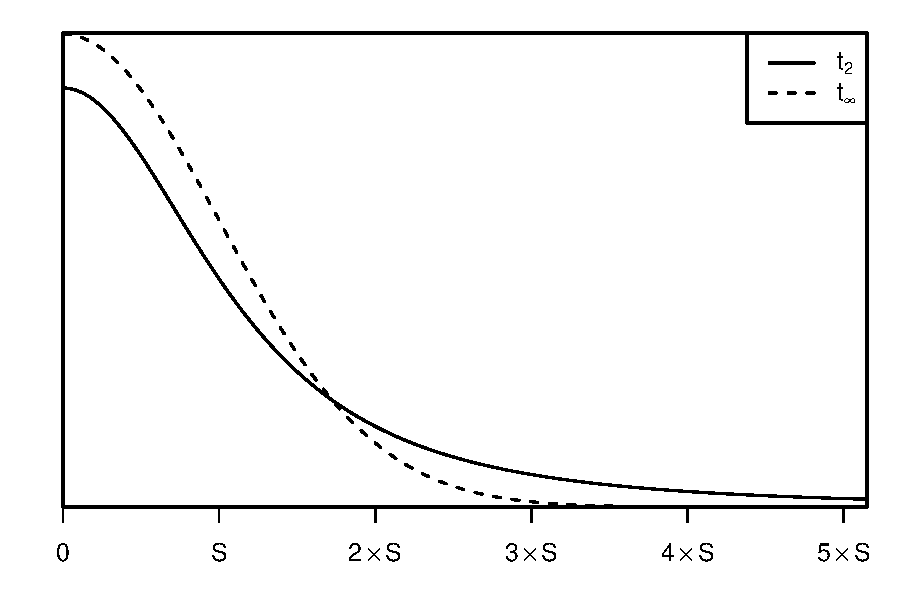
\includegraphics{figures/halft.pdf}
}
\caption{The half-t distribution with scale $S$ and 2 degrees of
  freedom (solid line). The dotted line shows the limit as the
  degrees of freedom increases to infinity \label{figure:halft}}
\end{figure}

\subsubsection{Scaled Wishart: \texttt{dscaled.wishart}}

The scaled Wishart distribution is defined by
\begin{verbatim}
Omega[1:M,1:M] ~ dscaled.wishart(s[1:M], df)
\end{verbatim}
where $s$ is a vector of prior scales of length $M$, $df$ is the
degrees of freedom, and $\Omega$ (Omega) is an $M \times M$ positive
definite symmetric matrix (If you want all elements to have the
same prior scale then use \texttt{rep(s, M)} as the first parameter).

The scaled Wishart is a multivariate generalization of the scaled
gamma distribution. It was proposed by \citet{HuangWand2013} as a flexible
family of prior distributions for the precision parameter of the
multivariate normal. When used in this way, the
\texttt{dscaled.wishart} distribution implicitly defines a prior on
the variance-covariance matrix $\Sigma = \Omega^{-1}$ with two
important features:
\begin{enumerate}
\item Let $\sigma_i = (\Sigma_{ii})^{1/2}$ be the standard deviation of
  element $i$ of the multivariate normal. Then $\sigma_i$ has a
  half-t distribution with scale $s_i$ and $df$ degrees of freedom
\item Let $\rho_{ij} = \Sigma_{ij}/(\sigma_i \sigma_j)$ for $i \neq j$
  be the correlation between elements $i$ and $j$ of the multivariate
  normal. For $df=2$, all correlation parameters $\rho_{ij}$ have a
  marginal uniform prior distribution. Larger values of $df$
  concentrate the prior around $\rho_{ij} = 0$.
\end{enumerate}


\section{Samplers in the glm module}
\label{section:glm::samplers}

The \verb+glm+ module implements samplers for efficient updating of
generalized linear mixed models.  The fundamental idea is to do block
updating of the parameters in the linear predictor.  The \verb+glm+
module is built on top of the \textsf{Csparse} and \textsf{CHOLMOD}
sparse matrix libraries \citep{Davis2006, Davis1999} which allows
updating of both fixed and random effects in the same
block. Currently, the methods only work on parameters that have a
normal prior distribution.

Some of the samplers are based in the idea of introducing latent
normal variables that reduce the GLM to a linear model. This idea was
introduced by \citet{AlbertChib93} for probit
regression with a binary outcome, and was later refined and extended
to logistic regression with binary outcomes by 
\citet{HolmesHeld06}. Another approach, auxiliary mixture sampling,
was developed by 
\citet{Fruhwirth-Schnatter09} and is used for more general Poisson
regression and logistic regression models with binomial outcomes.
\citet{Gamerman97} proposed a stochastic version of the iteratively
weighted least squares algorithm for GLMs, which is also implemented
in the \verb+glm+ module. However the IWLS sampler tends to break down
when there are many random effects in the model. It uses
Metropolis-Hastings updates, and the acceptance probability may be
very small under these circumstances.

Block updating in GLMMs frees the user from the need to center
predictor variables, like this:
\begin{verbatim}
y[i] ~ dnorm(mu[i], tau)
mu[i] <- alpha + beta * (x[i] - mean(x))
\end{verbatim}
The second line can simply be written
\begin{verbatim}
mu[i] <- alpha + beta * x[i]
\end{verbatim}
without affecting the mixing of the Markov chain.  

\chapter{The mix module}

%      Beta & \verb+dbetabin(a, b, n)+ &
%     \multirow{2}{*}{
%        $\textstyle {a+x-1 \choose x} {b+n-x-1 \choose n - x} 
%                    {a+b+n-1 \choose n}^{-1}$
%      } & $0$ & $n$ \\
%      binomial & $a > 0, b > 0, n \in \mathbb{N}^*$ \\

The \texttt{mix} module defines a novel distribution
\verb+dnormmix(mu,tau,pi)+ representing a finite mixture of normal
distributions. In the parameterization of the \verb+dnormmix+
distribution, $\mu$, $\tau$, and $\pi$ are vectors of the same length,
and the density of \verb+y ~ dnormmix(mu, tau, pi)+ is
\[
f(y | \mu, \tau, \pi) = \sum_i \pi_i \tau_i^{\frac{1}{2}} \phi( \tau^{\frac{1}{2}}_i (y - \mu_i))
\]
where $\phi()$ is the probability density function of a standard
normal distribution.

The \verb+mix+ module also defines a sampler that is designed to act
on finite normal mixtures. It uses tempered transitions to jump
between distant modes of the multi-modal posterior distribution
generated by such models \citep{Neal94,Celeux99}. The tempered
transition method is computationally very expensive. If you want to
use the \verb+dnormmix+ distribution but do not care about label
switching, then you can disable the tempered transition sampler with
\begin{verbatim}
set factory "mix::TemperedMix" off, type(sampler)
\end{verbatim}

\chapter{The dic module}

The \verb+dic+ module defines new monitor classes for Bayesian model
criticism using deviance-based measures. 

\subsection{The deviance monitor}

The deviance monitor records the deviance of the model ({\em i.e.} the
sum of the deviances of all the observed stochastic nodes) at each
iteration. The command
\begin{verbatim}
monitor deviance
\end{verbatim}
will create a deviance monitor {\em unless} you have defined a node
called ``deviance'' in your model. In this case, you will get a trace
monitor for your deviance node.

\subsection{The \texttt{pD} monitor}

The \verb+pD+ monitor is used to estimate the effective number of
parameters ($p_D$) of the model \citep{spiegelhalter:etal:2002}. It
requires at least two parallel chains in the model, but calculates
a single estimate of $p_D$ across all chains \citep{plummer:2002}.
A pD monitor can be created using the command:
\begin{verbatim}
monitor pD
\end{verbatim}
Like the deviance monitor, however, if you have defined a node called
``pD'' in your model then this will take precedence, and you will get
a trace monitor for your \verb+pD+ node.

Since the $p_D$ monitor pools its value across all chains, its values
will be written out to the index file ``CODAindex0.txt'' and
output file ``CODAoutput0.txt'' when you use the CODA command.

The effective number of parameters is the sum of separate contributions
from all observed stochastic nodes: $p_D = \sum_i p_{D_i}$. There is
also a monitor that stores the sample mean of $p_{D_i}$. These statistics
may be used as influence diagnostics \citep{spiegelhalter:etal:2002}.
The mean monitor for $p_{D_i}$ is created with:
\begin{verbatim}
monitor pD, type(mean)
\end{verbatim}
Its values can be written out to a file ``PDtable0.txt'' with
\begin{verbatim}
coda pD, type(mean) stem(PD)
\end{verbatim}

\subsection{The \texttt{popt} monitor}

The \verb+popt+ monitor works exactly like the mean monitor for $p_D$,
but records contributions to the optimism of the expected deviance
($p_{opt_i}$). The total optimism $p_{opt} = \sum_i p_{opt_i}$  can be
added to the mean deviance to give the penalized expected deviance
\citep{plummer:2008}.

The mean monitor for $p_{opt_i}$ is created with
\begin{verbatim}
monitor popt, type(mean)
\end{verbatim}
Its values can be written out to a file ``POPTtable0.txt'' with
\begin{verbatim}
coda popt, type(mean) step(POPT)
\end{verbatim}
Under asymptotically favourable conditions in which $p_{D_i} \ll 1
\forall i$,
\[
p_{opt} \approx 2 p_D
\]
For generalized linear models, a better approximation is
\[
p_{opt} \approx \sum_{i=1}^n \frac {p_{D_i}}{1 - p_{D_i}}
\]

The \verb+popt+ monitor uses importance weights to estimate
$p_{opt}$. The resulting estimates may be numerically unstable when
$p_{D_i}$ is not small.  This typically occurs in random-effects
models, so it is recommended to use caution with the \verb+popt+
until I can find a better way of estimating $p_{opt_i}$.

\chapter{The msm module}

The \verb+msm+ module defines the matrix exponential function
\verb+mexp+ and the multi-state distribution \verb+dmstate+ which
describes the transitions between observed states in continuous-time
multi-state Markov transition models. 

\chapter{Differences between \JAGS\ and \OpenBUGS}

Although \JAGS\ aims for the same functionality as \OpenBUGS, there are
a number of important differences.

\section{Data format}

There is no need to transpose matrices and arrays when transferring
data between \R\ and \JAGS, since \JAGS\ stores the values of an array
in ``column major'' order, like \R\ and FORTRAN ({\em i.e.} filling
the left-hand index first).

If you have an \textsf{S}-style data file for \OpenBUGS\ and you wish
to convert it for \JAGS, then use the command \texttt{bugs2jags},
which is supplied with the \CODA\ package.

\section{Distributions}

Structural zeros are allowed in the Dirichlet distribution. If
\begin{verbatim}
p ~ ddirch(alpha)
\end{verbatim}
and some of the elements of alpha are zero, then the corresponding
elements of p will be fixed to zero.

The Multinomial (\verb+dmulti+) and Categorical (\verb+dcat+)
distributions, which take a vector of probabilities as a parameter,
may use unnormalized probabilities. The probability vector is
normalized internally so that
\[
p_i \rightarrow \frac{p_i}{\sum_j p_j}
\]

The non-central hypergeometric distribution (\verb+dhyper+) uses the
same parameterization as R, which is different from the
parameterization used in OpenBUGS 3.2.2. OpenBUGS is parameterized as
\begin{verbatim}
X ~ dhyper(n, m, N, psi)     #OpenBUGS
\end{verbatim}
where $n, m, N$ are the following table margins:
\begin{center}
\begin{tabular}{|cc|c|}
\hline
x & - & n \\
-  & - & -  \\
\hline
m & - & N \\
\hline
\end{tabular}
\end{center}
This parameterization is symmetric in $n$, $m$. In JAGS, \verb+dhyper+
is parameterized as
\begin{verbatim}
X ~ dhyper(n1, n2, m1, psi) #JAGS 
\end{verbatim}
where $n1, n2, m1$ are
\begin{center}
\begin{tabular}{|cc|c|}
\hline
x & - & m1 \\
-  & - & -   \\
\hline
n1 & n2 & - \\
\hline
\end{tabular}
\end{center}

\section{Functions}

The \verb+max()+ and \verb+min()+ functions work like the
corresponding \R\ functions. They take a variable number of arguments
and return the maximum/minimum element over all supplied
arguments. This usage is  compatible with \OpenBUGS, although more general.

The \texttt{rank} function is distinct from \OpenBUGS, which has two
scalar-valued functions \verb+rank+ and \verb+ranked+.


\chapter{Acknowledgments}

Many thanks to the \BUGS\ development team, without whom \JAGS\ would
not exist.  Thanks also to Simon Frost for pioneering \JAGS\ on
Windows and Bill Northcott for getting \JAGS\ on Mac OS X to
work. Kostas Oikonomou found many bugs while getting \JAGS\ to work on
Solaris using Sun development tools and libraries.  Bettina Gruen,
Chris Jackson, Greg Ridgeway and Geoff Evans also provided useful
feedback.  Special thanks to Jean-Baptiste Denis who has been very
diligent in providing feedback on JAGS.

\appendix
\chapter{Data format}
\label{appendix:data}

The file format used by JAGS for representing data and initial values
is the \verb+dump()+ format used by R.  This format is valid R code,
so a JAGS data file can be read into R using the \verb+source()+ function.
Since R is a functional language, the code consists of a sequence
of assignments and function calls.
\begin{description}
\item[Assignments] are represented by a left arrow (\verb+<-+) with
  the variable name on the left hand side and a numeric value or
  function call on the right hand side. The variable name may
  optionally be enclosed in single quotes, double quotes, or back-ticks.
\item[Function calls] are represented by the function name, followed
  by a list of comma-separated arguments inside round brackets.
  Optional arguments need to be tagged (i.e. given in the form
  tag=value).
\end{description}
The \JAGS\ parser ignores all white space.  Long expressions can
therefore be split over several lines.

Scalar values are represented by a simple assignment statement 
\begin{verbatim}
theta <- 0.1243
\end{verbatim}
All numeric values are read in to JAGS as doubles, even if they are
represented as integers (i.e. `12' and `12.0' are
equivalent). Engineering notation may be used to represent large or
small values (e.g 1.5e-3 is equivalent to 0.0015).

Vectors are denoted by the \R\ collection function ``c'', which takes
a number of arguments equal to the length of the vector.  The
following code denotes a vector of length 4:
\begin{verbatim}
x <- c(2, 3.5, 1.3e-2, 88)
\end{verbatim}
There is no distinction between row and column-vectors. 

Matrices and higher-dimensional arrays in R are created by adding a
dimension attribute (\verb+.Dim+) to a vector. In the R dump format
this is done using the ``structure'' function.  The first argument to
the structure function is a vector of numeric values of the matrix,
given in column major order (i.e. filling the left index first). The
second argument, which must be given the tag \verb+.Dim+, is the
number of dimensions of the array, represented by a vector of integer
values. For example, if the matrix ``A'' takes values
\[
\left(
\begin{array}{cc}
  1 & 4 \\
  2 & 5 \\
  3 & 6 
\end{array}
\right)
\]
it is represented as
\begin{verbatim}
`A` <- structure(c(1, 2, 3, 4, 5, 6), .Dim=c(3,2))
\end{verbatim}

The simplest way to prepare your data is to read them into \R\ and
then dump them.  Only numeric vectors, matrices and arrays are
allowed. More complex data structures such as factors, lists and data
frames cannot be parsed by \JAGS\, nor can non-numeric vectors.  Any
\R\ attributes of the data (such as names and dimnames) are ignored
when they are read into \JAGS. 

\bibliographystyle{abbrvnat}
\bibliography{jags_user_manual}

\end{document}



